\chapter{Testes e Resultados}
% Revisar

Os testes de infraestrutura desempenham um papel fundamental na garantia de que uma plataforma está pronta para ser utilizada em produção. Eles permitem verificar e validar aspectos cruciais da infraestrutura, como escalabilidade, tolerância a falhas, desempenho e segurança. Garantir que esses elementos estão funcionando conforme o esperado é essencial para proporcionar uma experiência de usuário satisfatória e para manter a integridade e disponibilidade da plataforma.

Neste capítulo, serão apresentados os testes realizados na plataforma Codeboard UERJ, com o objetivo de avaliar e validar sua escalabilidade, tolerância a falhas, desempenho e segurança. Os testes foram conduzidos em um ambiente de produção, visando simular situações reais de uso e identificar possíveis pontos de melhoria na infraestrutura.


\section{Distribuição de Carga}
% OK (revisar?)

Para avaliar a distribuição de carga em diferentes níveis da infraestrutura da plataforma Codeboard UERJ, foram realizadas modificações no código-fonte, permitindo a coleta de informações detalhadas sobre a máquina que processa cada requisição, como o identificador da instância EC2 na AWS e o identificador do processo (PID) responsável pelo processamento da requisição. Com esses dados, foi possível analisar como a carga está sendo distribuída entre diferentes regiões geográficas, servidores e processos.

\subsection{Balanceamento de Carga entre Regiões Geográficas}
% OK (revisar?)

Para avaliar a eficiência do balanceamento de carga entre diferentes regiões geográficas, realizamos testes simulando acessos à plataforma a partir de máquinas virtuais localizadas em diversas partes do mundo. Essas simulações foram projetadas para identificar o comportamento da infraestrutura em termos de roteamento e tempo de resposta.

Foram utilizadas máquinas virtuais em quatro regiões: Brasil, Estados Unidos, Ásia e Oceania. Cada máquina realizou 100 requisições à rota \texttt{/api/health}, e os dados coletados incluíram informações como o IP do servidor que processou cada requisição e o tempo médio de resposta. O IP foi utilizado para determinar a região geográfica do servidor responsável, possibilitando uma análise detalhada da distribuição de carga.

A Tabela \ref{tab:geo-distribution} apresenta os resultados dos testes, destacando como as requisições foram distribuídas entre os servidores. A análise revelou que as requisições originadas no Brasil e nos Estados Unidos foram roteadas para seus respectivos servidores locais, resultando em uma latência significativamente menor para os usuários dessas regiões. Em contraste, as requisições provenientes da Ásia e da Oceania foram processadas pelo servidor localizado nos Estados Unidos, o que gerou tempos de resposta mais elevados devido à distância geográfica.

\begin{table}[H]
    \centering
    \caption{Resultados dos testes de distribuição de carga entre diferentes regiões geográficas}
    \label{tab:geo-distribution}
    \begin{tabular}{|l|l|l|}
        \hline
        \textbf{Origem}   & \textbf{Servidor Designado} & \textbf{Latência média} \\ \hline
        Brasil         & Brasil                      & 185 ms                  \\ \hline
        Estados Unidos & Estados Unidos              & 164 ms                  \\ \hline
        Ásia           & Estados Unidos              & 412 ms                  \\ \hline
        Oceania        & Estados Unidos              & 378 ms                  \\ \hline
    \end{tabular}
\end{table}

Embora essa configuração atenda bem às necessidades das regiões próximas, a latência elevada observada para a Ásia e Oceania sugere que a adição de servidores em novas regiões poderia melhorar significativamente a experiência do usuário. Essa expansão reduziria a distância física entre os usuários e os servidores, promovendo um balanceamento de carga mais eficiente e tempos de resposta mais baixos em escala global.


\subsection{Balanceamento de Carga entre Servidores}
% OK (revisar?)

Para avaliar o balanceamento de carga entre servidores dentro de uma mesma região, realizamos 5000 requisições à rota \texttt{/api/health} a partir da região geográfica do Brasil. Com as modificações feitas no código da plataforma, foi possível coletar as informações sobre qual servidor processou cada requisição.

Os resultados dos testes estão apresentados na Figura \ref{fig:reqs-per-instance} e na Figura \ref{fig:reqs-per-instance-over-time}, que mostram respectivamente a distribuição de carga entre diferentes servidores e a distribuição ao longo do tempo. Os dados coletados incluem a quantidade de requisições processadas por cada servidor e a identificação do servidor responsável pelo processamento.

\begin{figure}[H]
    \centering
    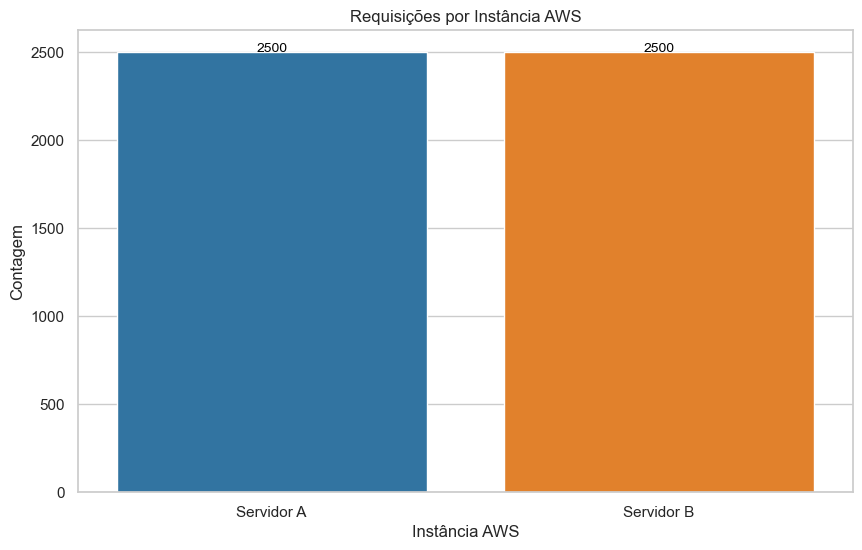
\includegraphics[width=1\textwidth]{assets/balance-test/reqs-per-instance.png}
    \caption{Distribuição de carga entre diferentes servidores}
    \label{fig:reqs-per-instance}
\end{figure}

\begin{figure}[H]
    \centering
    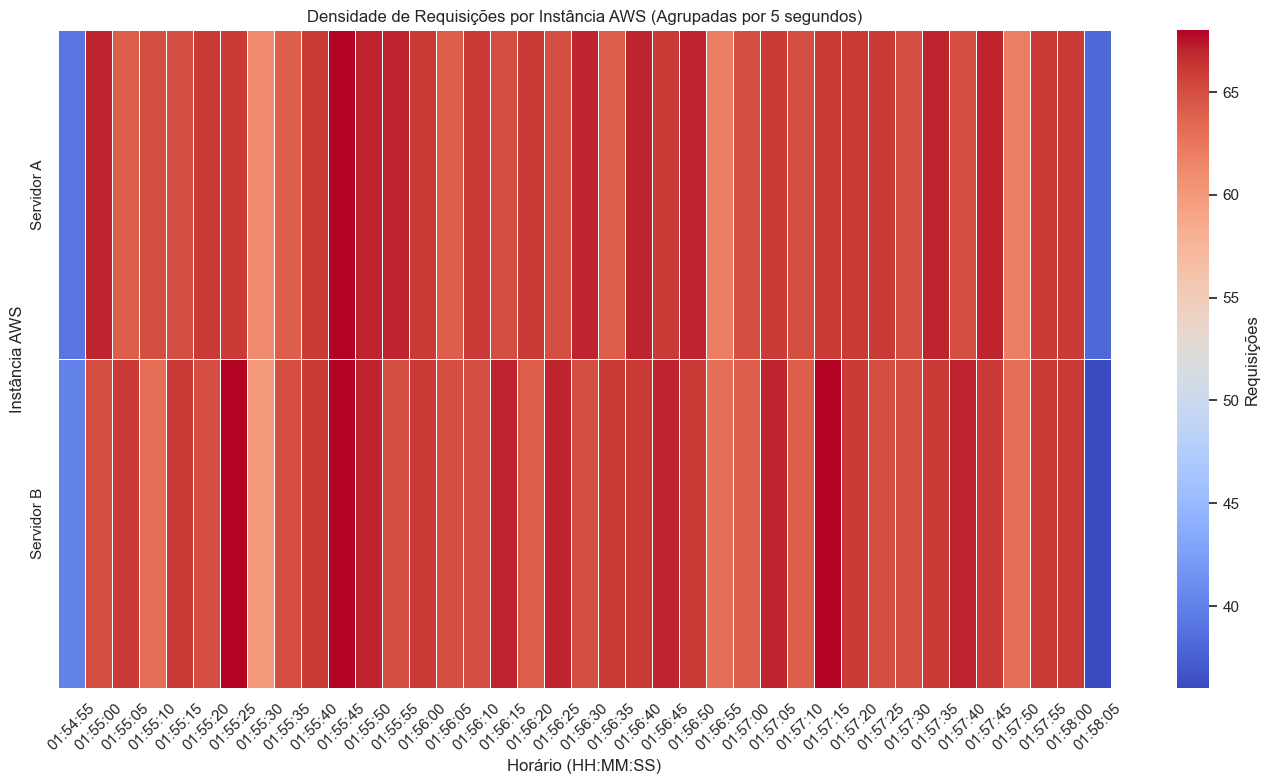
\includegraphics[width=1\textwidth]{assets/balance-test/reqs-per-instance-over-time.png}
    \caption{Distribuição de carga entre diferentes servidores ao longo do tempo}
    \label{fig:reqs-per-instance-over-time}
\end{figure}

Como pode ser observado na Figura \ref{fig:reqs-per-instance}, a distribuição de carga entre diferentes servidores foi realizada de forma eficiente, com metade das requisições sendo processadas por cada uma das instâncias disponíveis. O gráfico da Figura \ref{fig:reqs-per-instance-over-time} mostra que as requisições foram processadas de forma homogênea e alternada entre os dois servidores ao longo do tempo, validando a estratégia Round Robin utilizada para o balanceamento de carga entre diferentes servidores da infraestrutura.

Os dados indicam que o balanceador de carga distribuiu as requisições de forma equitativa entre os dois servidores disponíveis, validando a eficácia da estratégia de balanceamento utilizada. Essa distribuição contribuiu para uma utilização otimizada dos recursos presentes na infraestrutura e para a redução de possíveis gargalos de desempenho, evitando sobrecargas em um único servidor.

\subsection{Balanceamento de Carga entre Processos}
% OK (revisar!)

Para avaliar o balanceamento de carga entre processos dentro de um mesmo servidor, analisaremos novamente as 5000 requisições anteriormente realizadas para a rota \texttt{/api/health}. Desta vez, utilizamos também o identificador do processo (PID) em nossa analise para identificar qual processo foi responsável pelo processamento de cada requisição.

Os resultados estão apresentados na Figura \ref{fig:reqs-per-pid}, que mostra a distribuição de carga entre diferentes processos, e na Figura \ref{fig:reqs-per-pid-over-time}, que mostra a distribuição ao longo do tempo. Os dados coletados incluem a quantidade de requisições processadas por cada processo, a identificação do servidor e do PID responsável pelo processamento.


\begin{figure}[H]
    \centering
    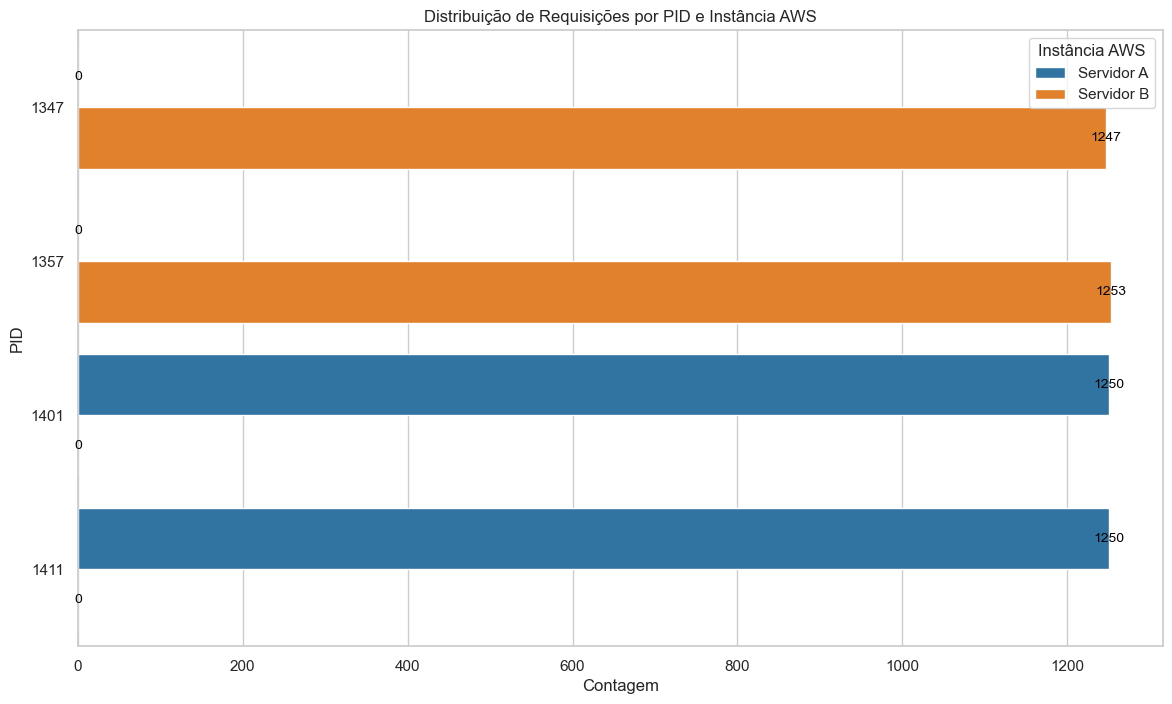
\includegraphics[width=1\textwidth]{assets/balance-test/reqs-per-pid.png}
    \caption{Distribuição de carga entre diferentes servidores}
    \label{fig:reqs-per-pid}
\end{figure}

\begin{figure}[H]
    \centering
    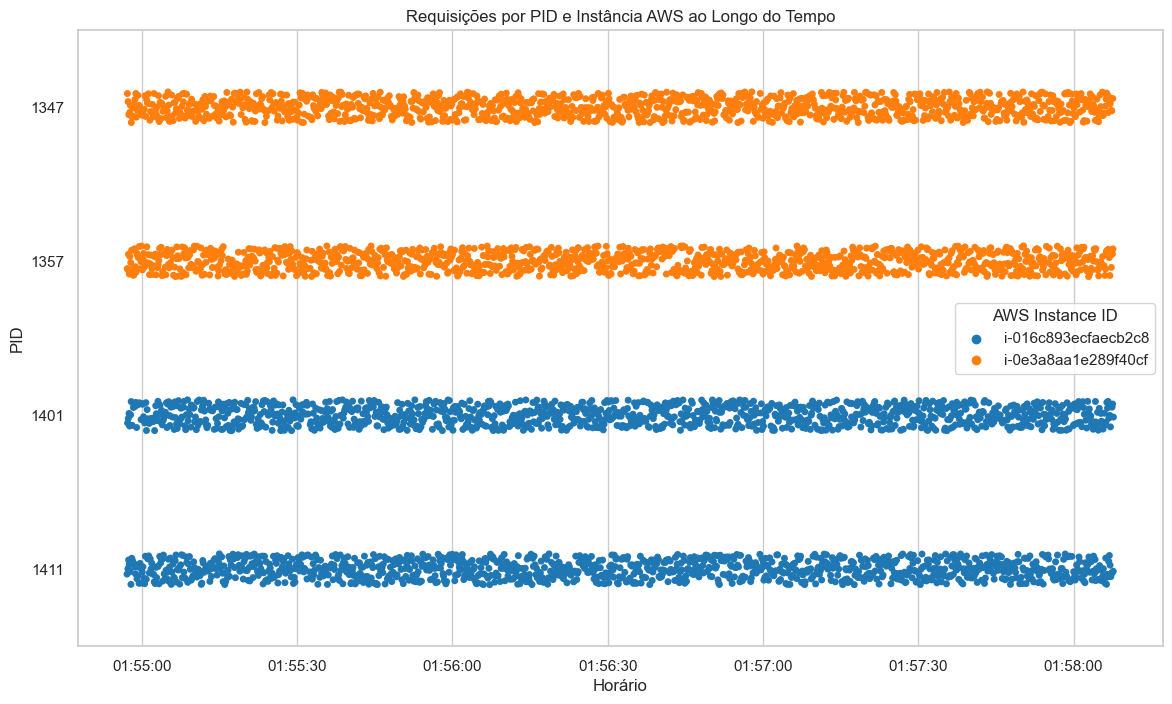
\includegraphics[width=1\textwidth]{assets/balance-test/reqs-per-pid-over-time.png}
    \caption{Distribuição de carga entre diferentes servidores ao longo do tempo}
    \label{fig:reqs-per-pid-over-time}
\end{figure}

Analisando os dados da Figura \ref{fig:reqs-per-pid}, observamos que as requisições foram distribuídas de forma quase que totalmente equilibrada entre os processos disponíveis, com uma pequena diferença entre a quantidade de requisições processadas por cada um. O gráfico da Figura \ref{fig:reqs-per-pid-over-time} mostra que as requisições foram processadas de forma homogênea entre os diferentes processos ao longo do tempo, validando a estratégia de balanceamento de carga utilizada entre os núcleos de processamento dos servidores.


\section{Testes de Elasticidade}
% OK (revisar?)

Esta seção apresenta os testes de elasticidade realizados na plataforma Codeboard UERJ. Os testes foram realizados com o objetivo de validar a capacidade da infraestrutura de suportar um grande volume de usuários simultâneos, analisando o desempenho do servidor back-end em diferentes cenários de uso. Os testes foram realizados com a infraestrutura provisionada com somente uma região geográfica, a do Brasil.


\subsection{Metodologia de Testes}

Os testes de elasticidade foram conduzidos utilizando a ferramenta Grafana K6 \cite{grafana-k6}, que permite simular um grande número de usuários acessando a plataforma simultaneamente. Configuramos a ferramenta para executar testes em etapas de carga progressiva, permitindo a medição de métricas como latência, taxa de erro e capacidade de resposta do sistema. Os testes foram divididos em três etapas principais:

\begin{enumerate}
    \item \textbf{Subida inicial:} Durante 10 minutos, o número de usuários simultâneos aumentou gradualmente até atingir 300.
    \item \textbf{Manutenção da carga:} O sistema manteve 300 usuários simultâneos por um período de 5 minutos.
    \item \textbf{Redução da carga:} A carga foi reduzida gradualmente para 0 ao longo de 5 minutos.
\end{enumerate}

Cada usuário simulado seguiu um fluxo típico de interação com a plataforma Codeboard UERJ, composto por cinco etapas principais: login, criação de sala, entrada na sala, codificação colaborativa e desconexão. Cada etapa envolveu a execução de requisições HTTP e comunicação via WebSocket, simulando o comportamento de um usuário real na plataforma.

\begin{enumerate}
    \item \textbf{Login:} Os usuários simulados iniciaram o fluxo realizando login na plataforma pela rota \texttt{/api/auth/login} utilizando credenciais válidas préviamente criadas no banco de dados. Após a autenticação, cada usuário recebeu um token JWT, essencial para acessar as funcionalidades subsequentes.
    \item \textbf{Criação de Sala:} Com o login concluído, os usuários criaram salas por meio da rota \texttt{/api/rooms}. Cada sala foi identificada por um nome único, e a API retornou um identificador correspondente à sala criada.
    \item \textbf{Entrada na Sala:} Após a criação, os usuários entraram nas salas utilizando a rota \texttt{/api/room/:roomId}. Eles buscaram informações da sala e se conectaram ao servidor WebSocket utilizando o token JWT e o identificador da sala. Durante essa etapa, enviaram as mensagens \texttt{room:join} e \texttt{board:join} para indicar que estavam prontos para iniciar a codificação colaborativa.
    \item \textbf{Escrita de Código:} Na etapa de codificação, os usuários interagiram via WebSocket, trocando mensagens de texto representativas de ações de escrita de código. Para simulação, cada usuário enviou 10 mensagens \texttt{board:write}, com intervalos de 3 segundos entre elas. Essas mensagens foram processadas pelo servidor e redistribuídas aos demais participantes da sala.
    \item \textbf{Desconexão:} Ao final da simulação, os usuários finalizaram a sessão de codificação enviando as mensagens \texttt{room:leave} e \texttt{board:leave}. Em seguida, desconectaram-se do servidor WebSocket. O servidor então gerou mensagens em fila para serem processadas posteriormente, salvando o código escrito no banco de dados e concluindo o ciclo de interação do usuário com a plataforma.
\end{enumerate}


\subsection{Resultados dos Testes}

Os resultados obtidos demonstram que a infraestrutura da plataforma Codeboard UERJ respondeu adequadamente às demandas simuladas, ajustando-se ao aumento e à redução do número de usuários sem apresentar falhas críticas. A seguir, detalhamos os principais resultados obtidos durante os testes.

Na Figura \ref{fig:elasticity-vus-and-reqs}, observa-se o comportamento do número de usuários simultâneos e da taxa de requisições por segundo processadas durante o teste. Conforme descrito na metodologia, o número de usuários aumentou gradualmente até 300, permaneceu constante por 5 minutos e foi reduzido a 0. A taxa de requisições processadas acompanhou o aumento e a redução do número de usuários, indicando que o sistema foi capaz de lidar com a carga de forma eficiente.

\begin{figure}[H]
    \centering
    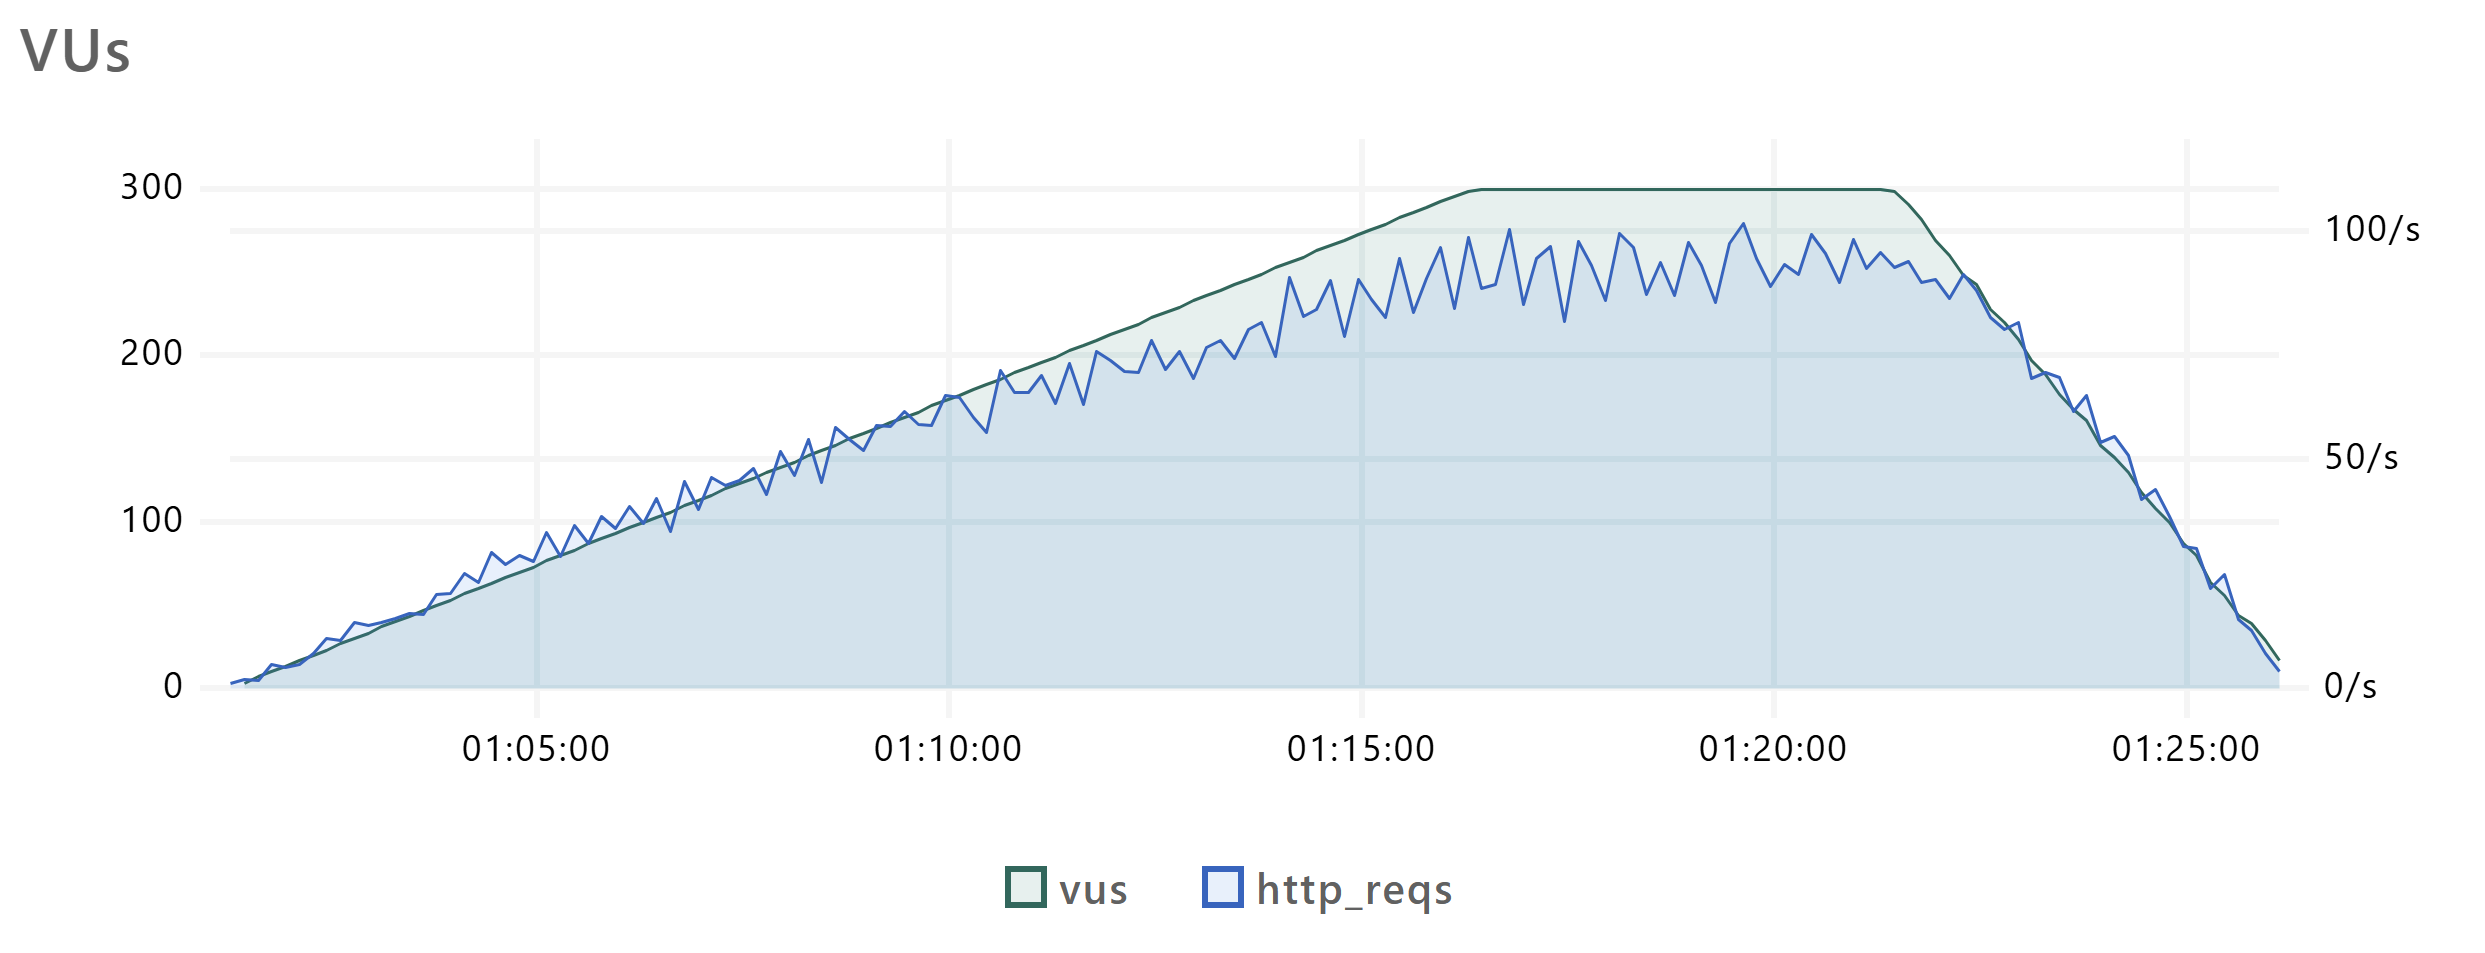
\includegraphics[width=1\textwidth]{assets/elasticity-test/vus-and-reqs.png}
    \caption{Número de usuários virtuais e taxa de requisições processadas por segundo ao longo do teste de elasticidade}
    \label{fig:elasticity-vus-and-reqs}
\end{figure}

A Figura \ref{fig:elasticity-req-duration} apresenta a média e o percentil 95 da duração das requisições durante o teste. A média iniciou em aproximadamente 250 ms e aumentou gradualmente à medida que o número de usuários crescia, alcançando um pico de 1,3 segundos. O percentil 95, que reflete o tempo das 5\% requisições mais lentas, chegou a um máximo de 3 segundos. Apesar do aumento na latência com a elevação da carga, os tempos de resposta permaneceram dentro de limites aceitáveis.

\begin{figure}[H]
    \centering
    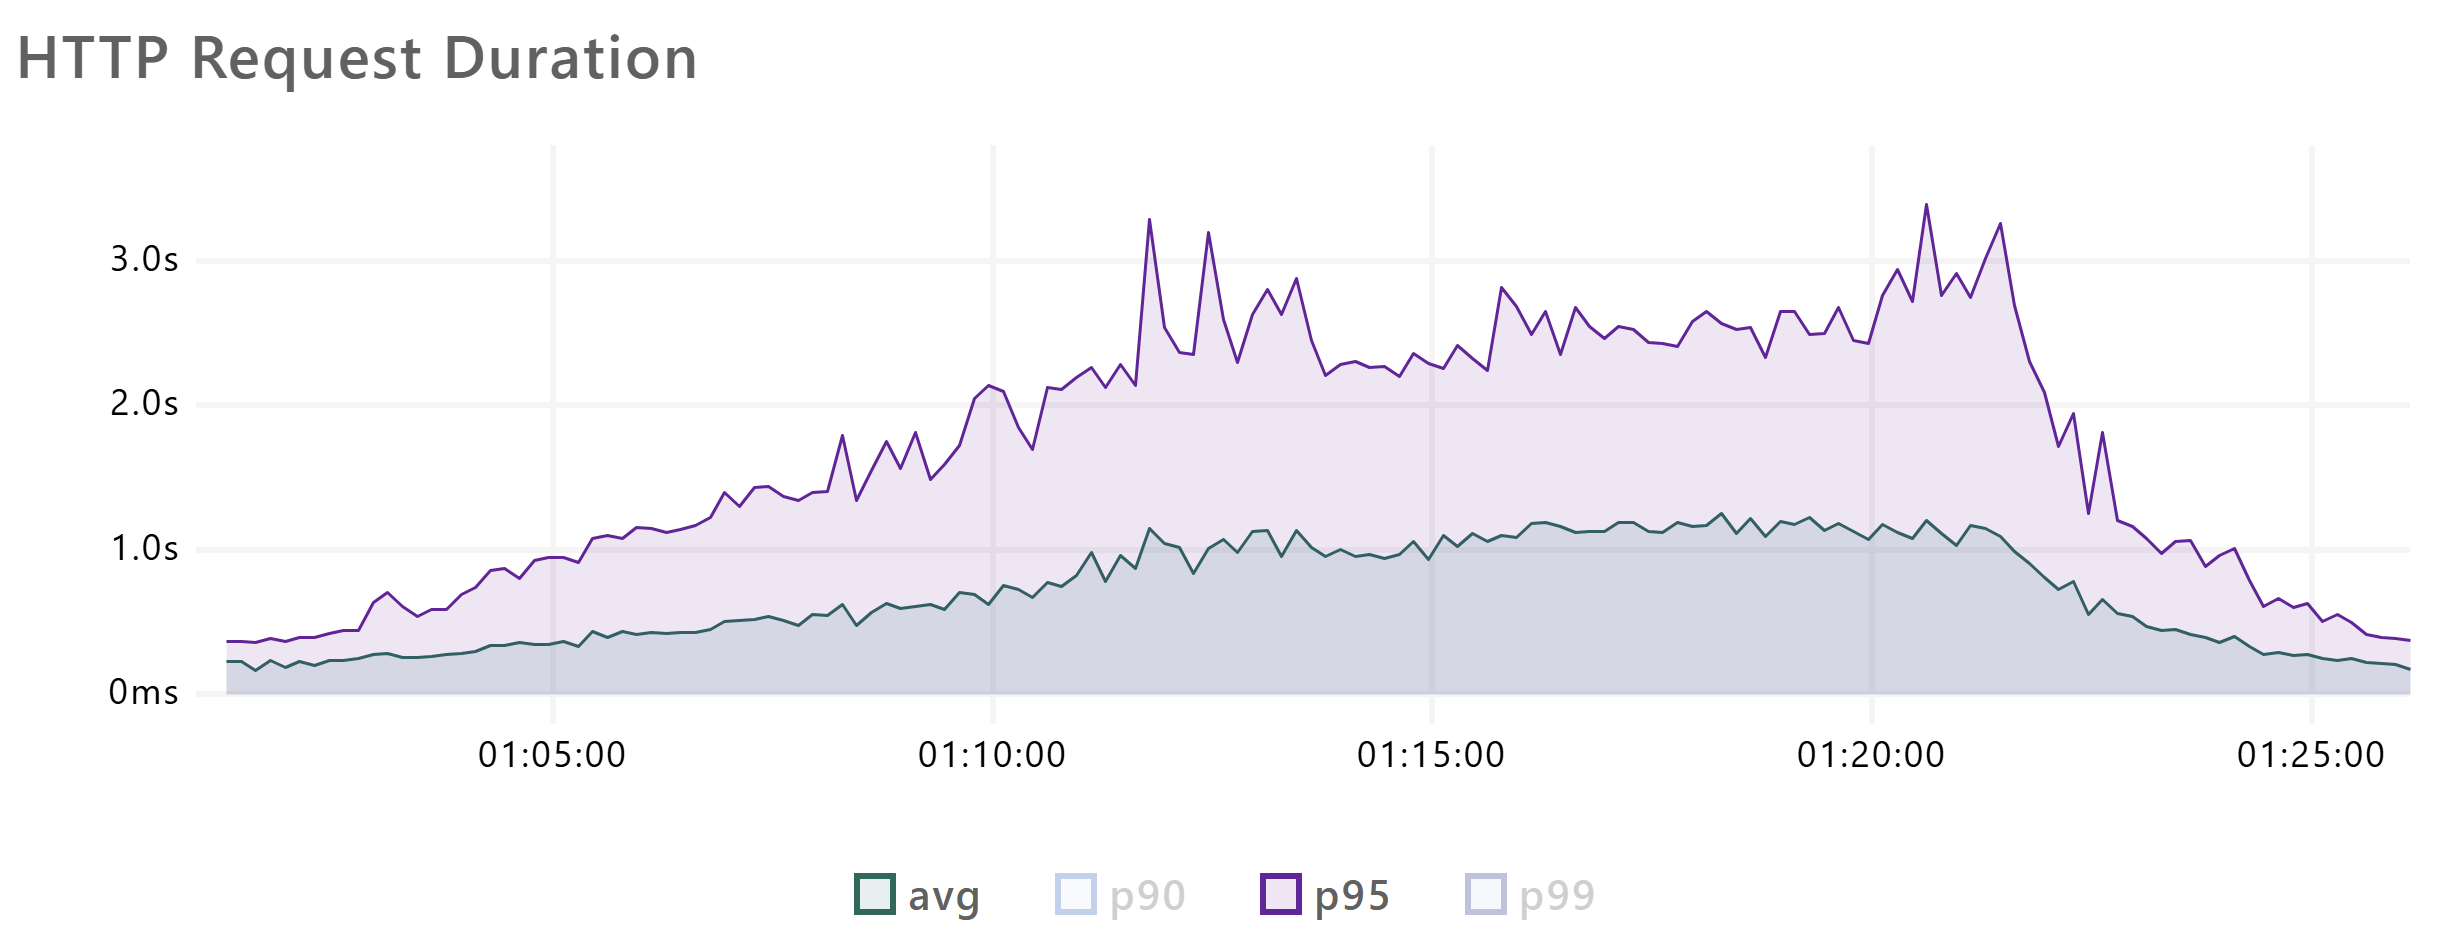
\includegraphics[width=1\textwidth]{assets/elasticity-test/req-duration.png}
    \caption{Duração das requisições ao longo do teste de elasticidade}
    \label{fig:elasticity-req-duration}
\end{figure}

A taxa de requisições falhadas, ilustrada na Figura \ref{fig:elasticity-req-failed-rate}, manteve-se em torno de 0,2 requisição por segundo, representando menos de 1\% do total processado. Esses resultados evidenciam a resiliência do sistema, que lidou bem com as demandas sem falhas críticas ou interrupções significativas no serviço.

\begin{figure}[H]
    \centering
    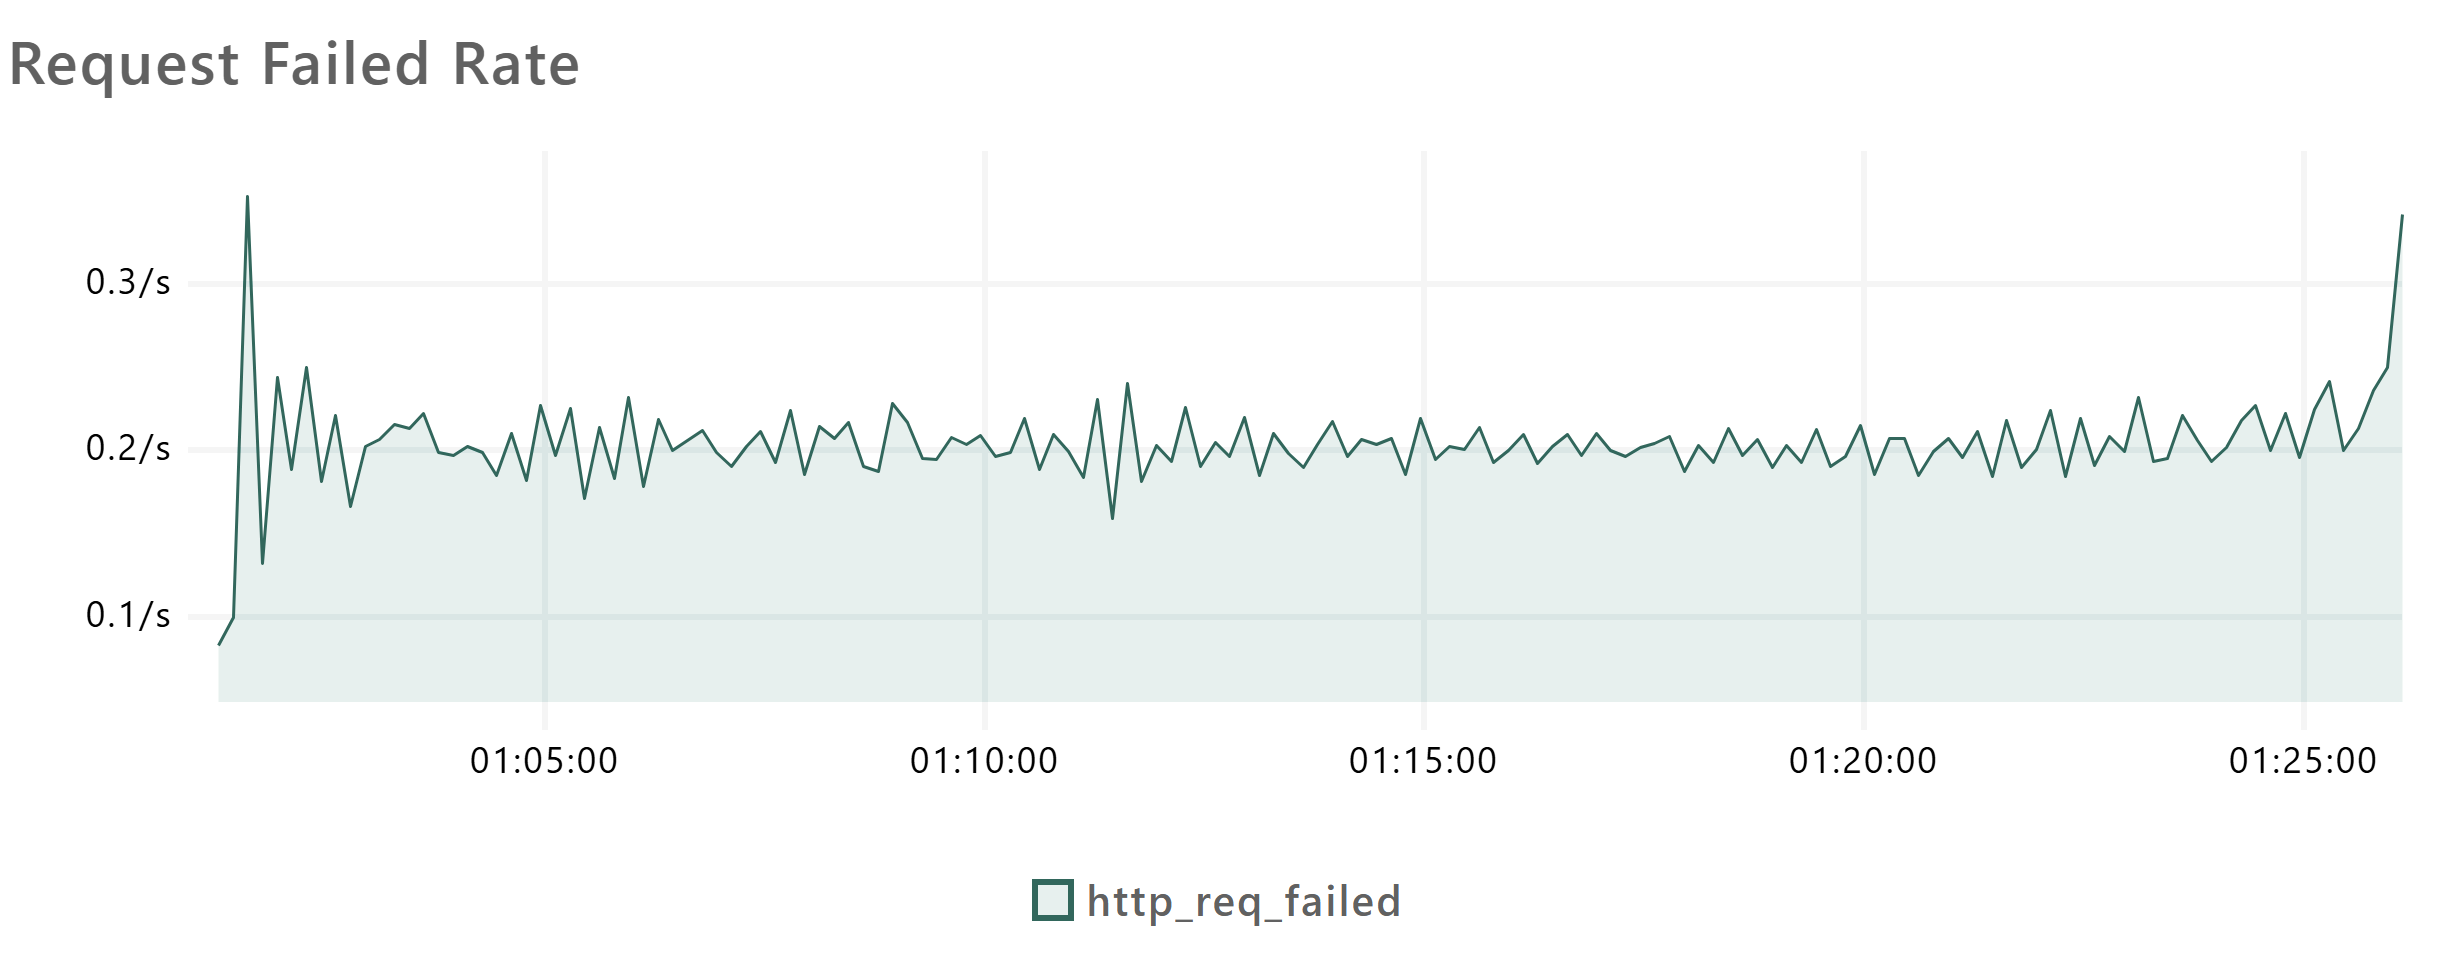
\includegraphics[width=1\textwidth]{assets/elasticity-test/req-failed-rate.png}
    \caption{Taxa de requisições falhadas ao longo do teste de elasticidade}
    \label{fig:elasticity-req-failed-rate}
\end{figure}

A Figura \ref{fig:elasticity-healthy-hosts} ilustra a evolução do número de servidores disponíveis durante o teste. Nos primeiros 10 minutos, quando o número de usuários era insuficiente para impactar a infraestrutura, a quantidade de servidores permaneceu constante em dois. À medida que o número de usuários se aproximava do pico de 300, um terceiro servidor foi adicionado à infraestrutura para atender à demanda adicional. Esse padrão se repetiu conforme o crescimento do tráfego, resultando em um pico de cinco servidores. Posteriormente, com a diminuição da carga e o término do teste, os servidores adicionais foram desativados, restabelecendo o estado inicial de dois servidores. Esse comportamento demonstra a capacidade do sistema de adaptar-se dinamicamente ao tráfego, escalando horizontalmente para atender a cargas mais elevadas e reduzindo a capacidade quando a demanda diminui.

\begin{figure}[H]
    \centering
    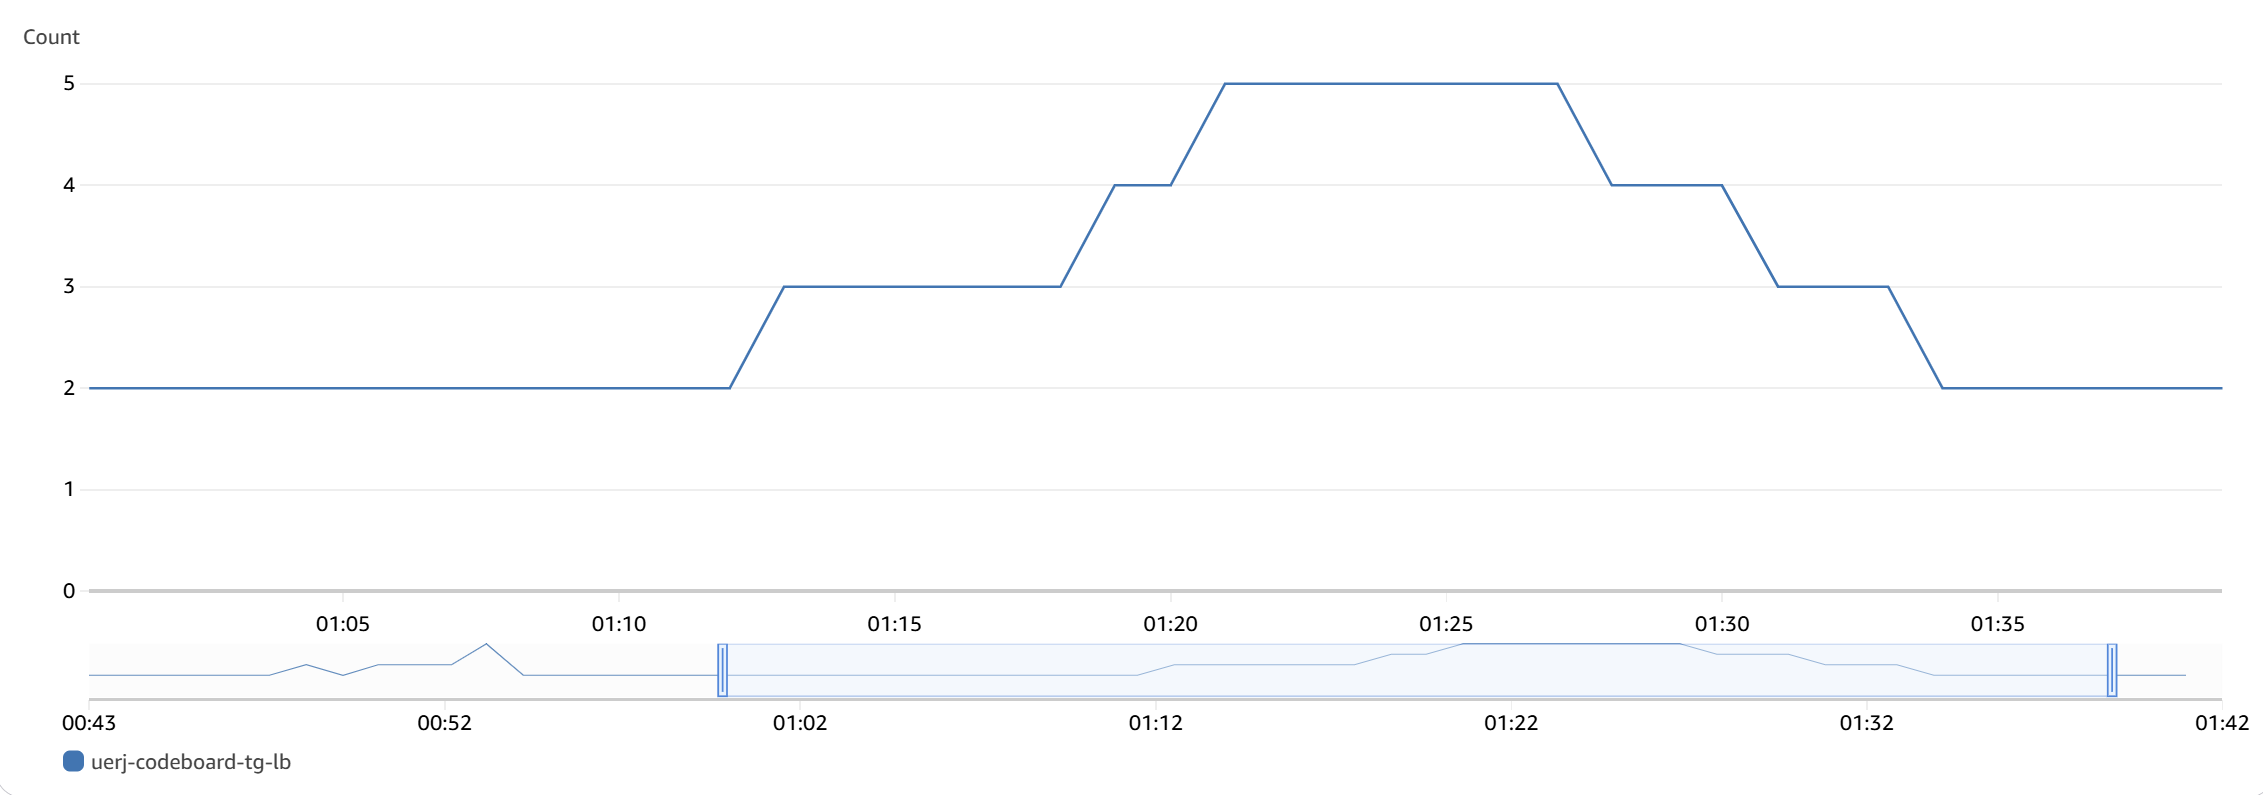
\includegraphics[width=1\textwidth]{assets/elasticity-test/healthy-hosts.png}
    \caption{Número de servidores disponíveis ao longo do teste de elasticidade}
    \label{fig:elasticity-healthy-hosts}
\end{figure}

Cabe ressaltar que o gráfico apresentado na Figura \ref{fig:elasticity-healthy-hosts} considera apenas os servidores disponíveis para processar requisições. O tempo de inicialização de novos servidores é de aproximadamente dois minutos. Por exemplo, o gatilho para a adição de um novo servidor ocorreu por volta de 01:11, mas ele somente se tornou operacional para processar requisições em 01:13, momento em que o gráfico passou a refletir sua presença.

Por fim, a Figura \ref{fig:elasticity-unhealthy-hosts} destaca que, durante o momento de maior estresse na infraestrutura, coincidindo com a provisão de um novo servidor, um dos servidores apresentou problemas de saúde. Isso indica que o servidor estava tão sobrecarregado que não conseguia processar sequer os healthchecks, levando o balanceador de carga a marca-lo temporariamente como não saudável. No entanto, com a adição de novos servidores poucos minutos depois, o servidor conseguiu se recuperar e retornar ao processamento de requisições. Esse padrão foi observado repetidamente conforme o aumento do número de usuários, demonstrando a capacidade da infraestrutura de se adaptar dinamicamente às demandas de tráfego.

\begin{figure}[H]
    \centering
    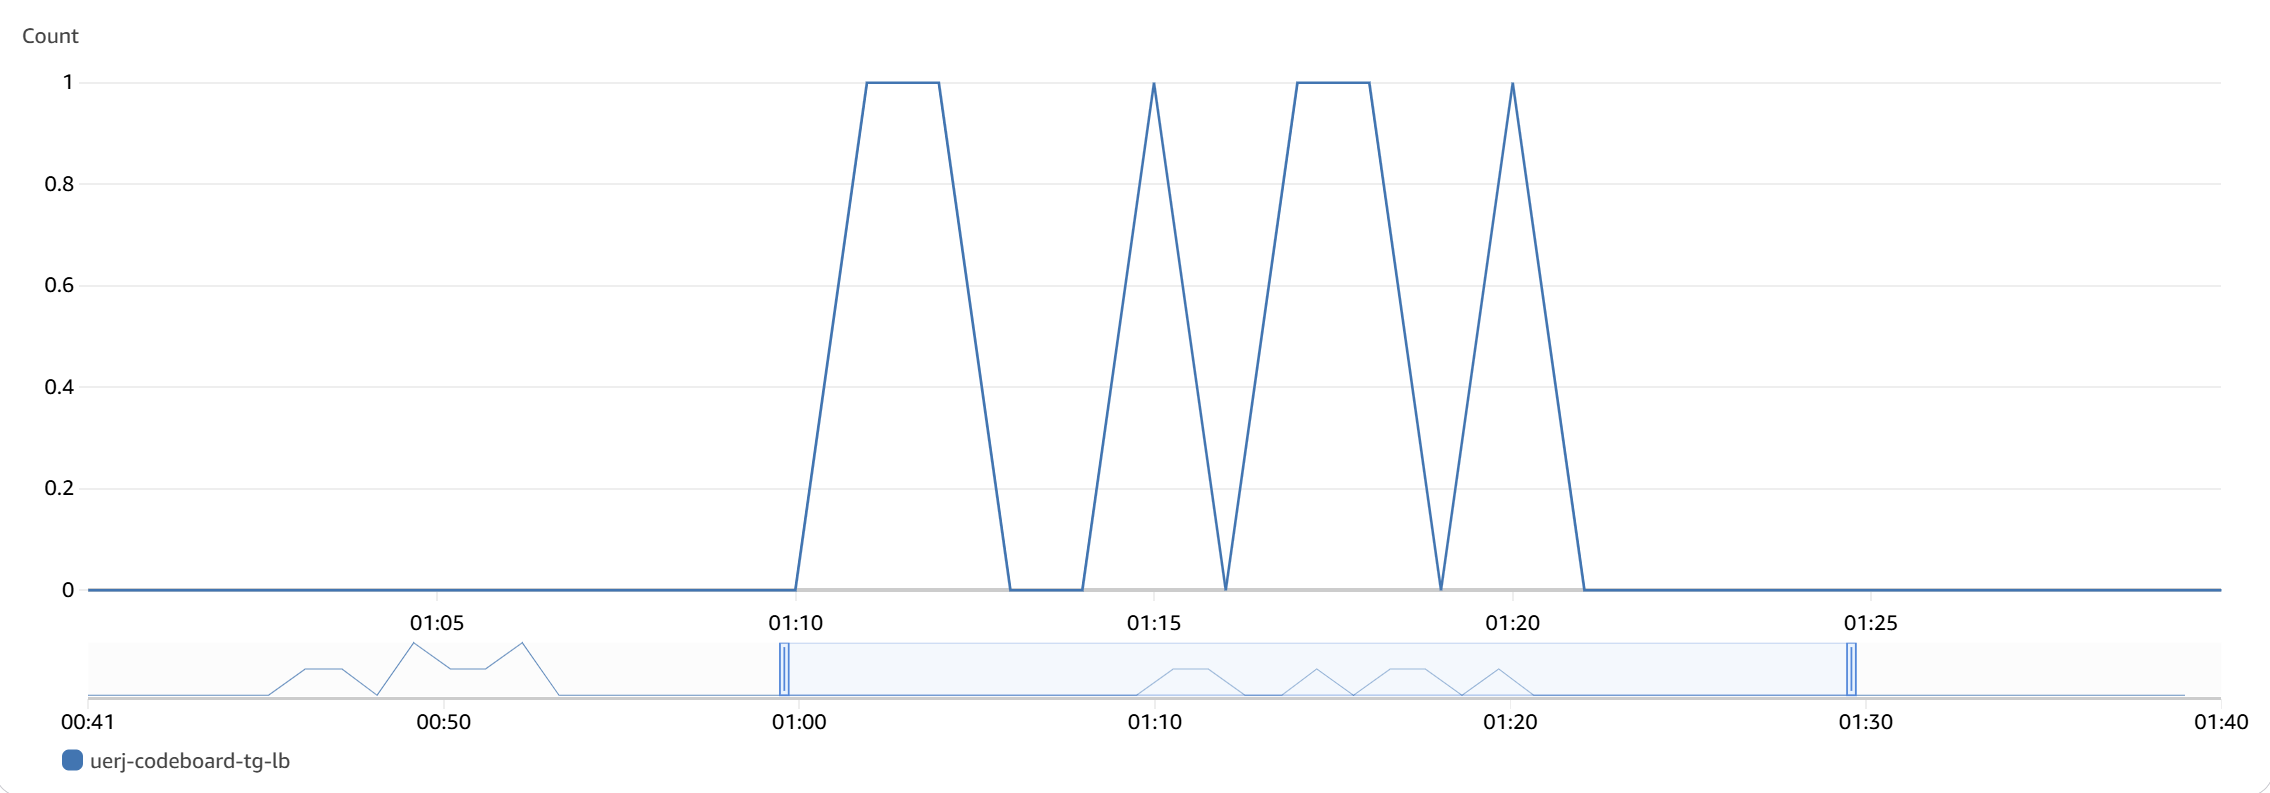
\includegraphics[width=1\textwidth]{assets/elasticity-test/unhealthy-hosts.png}
    \caption{Número de servidores não saudáveis ao longo do teste de elasticidade}
    \label{fig:elasticity-unhealthy-hosts}
\end{figure}


\section{Testes de Tolerância a Falhas}
% OK!

Nesta seção, apresentamos os testes de tolerância a falhas realizados na plataforma Codeboard UERJ. Os testes foram conduzidos com o objetivo de avaliar a capacidade da infraestrutura de se recuperar de falhas de servidores e processos de forma automática, garantindo a disponibilidade da plataforma em situações de falha.

\subsection{Metodologia de Testes}

Os testes de tolerância a falhas foram realizados de forma similar aos testes de elasticidade, mas com valores reduzidos para simular condições de uso mais estáveis e avaliar a capacidade de recuperação da infraestrutura em situações de falha. As etapas foram adaptadas com 30 usuários simultâneos e duração total de 15 minutos, divididas da seguinte forma:

\begin{enumerate}
    \item \textbf{Subida inicial:} Durante 3 minutos, o número de usuários simultâneos aumentou gradualmente até atingir 30.
    \item \textbf{Manutenção da carga:} O sistema manteve 30 usuários simultâneos por um período de 5 minutos.
    \item \textbf{Redução da carga:} A carga foi reduzida gradualmente para 0 ao longo de 3 minutos.
\end{enumerate}

Os testes foram conduzidos durante a etapa de manutenção da carga, com o objetivo de avaliar a capacidade da infraestrutura de se recuperar de falhas de servidores e processos de forma automática, garantindo a disponibilidade da plataforma em situações adversas. Durante os testes a infraestrutura estava provisionada inicialmente com dois servidores e somente uma região geográfica, a do Brasil.

\subsection{Falhas de Servidores}


Para avaliar a resiliência da infraestrutura em caso de falhas, realizamos a simulação de uma falha em um dos servidores. O teste envolveu o desligamento manual do servidor por meio do painel de controle da AWS, que permite a interrupção seja realizada de forma abrupta. A infraestrutura foi monitorada para verificar a capacidade de recuperação automática e a continuidade do serviço durante a falha.

A Figura \ref{fig:server-failing-vus-and-reqs} mostra a evolução do número de usuários simultâneos e da taxa de requisições processadas ao longo do teste. Conforme descrito na metodologia, o número de usuários foi gradualmente aumentado até 30, manteve-se constante por 5 minutos e, em seguida, foi reduzido a zero. Durante esse período, a taxa de requisições acompanhou esse comportamento, mas sofreu uma queda às 01:44:38 devido ao desligamento de um dos servidores. Após o reinício automático do servidor, às 01:45:40, a taxa de requisições voltou ao normal.

\begin{figure}[H]
    \centering
    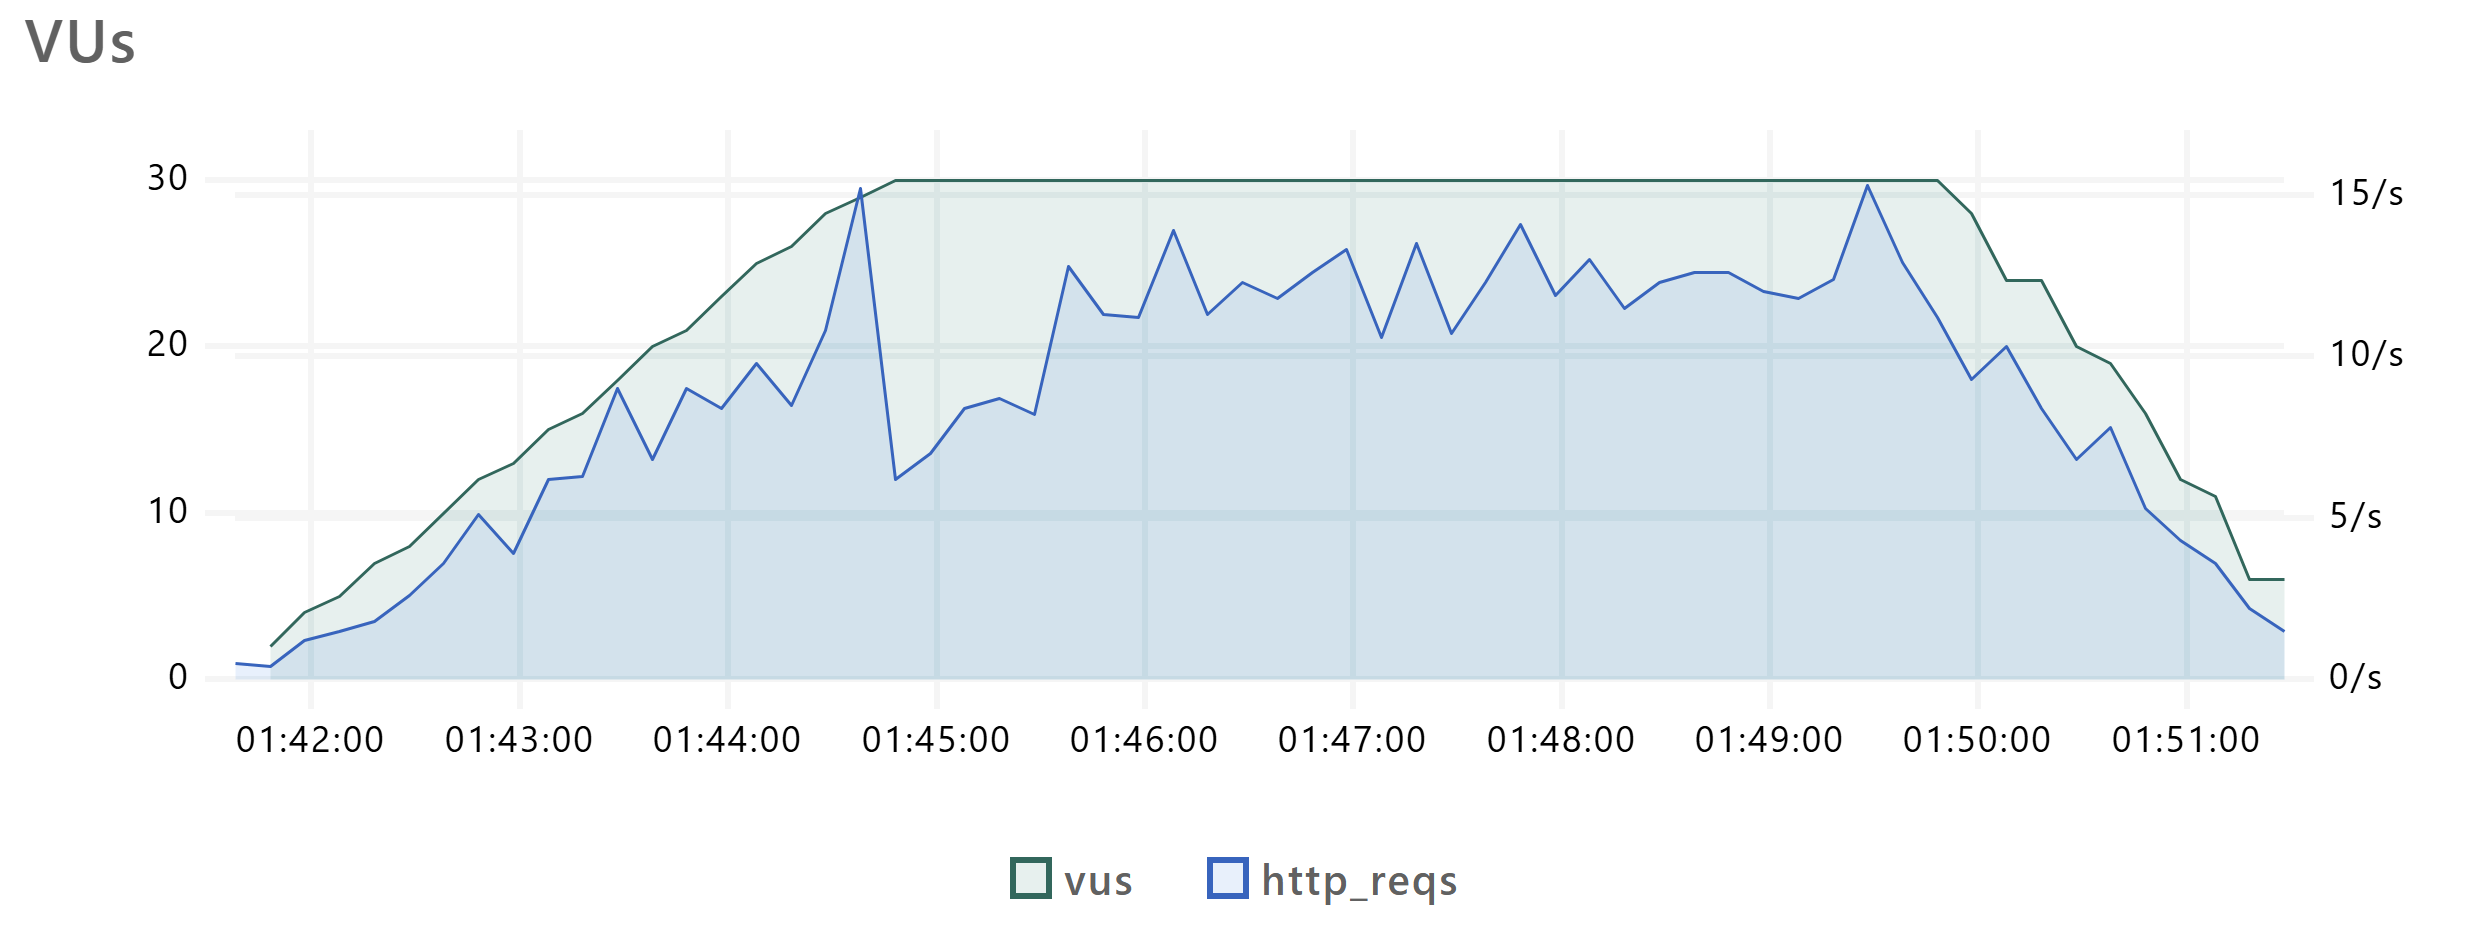
\includegraphics[width=1\textwidth]{assets/server-failing-test/vus-and-reqs.png}
    \caption{Número de usuários virtuais e taxa de requisições processadas por segundo ao longo do teste de falha de servidor}
    \label{fig:server-failing-vus-and-reqs}
\end{figure}

A Figura \ref{fig:server-failing-req-duration} apresenta a média e o percentil 95 das durações das requisições. Em condições normais, a média foi de aproximadamente 250 ms. Durante a falha, houve um aumento significativo, com a média atingindo 2 segundos e o percentil 95 alcançando 10 segundos. Por volta de 01:45:40, após a identificação da falha e o redirecionamento do tráfego para o servidor restante, os tempos de resposta retornaram aos valores normais, porém com uma leve oscilação devido ao aumento de carga no servidor restante.

\begin{figure}[H]
    \centering
    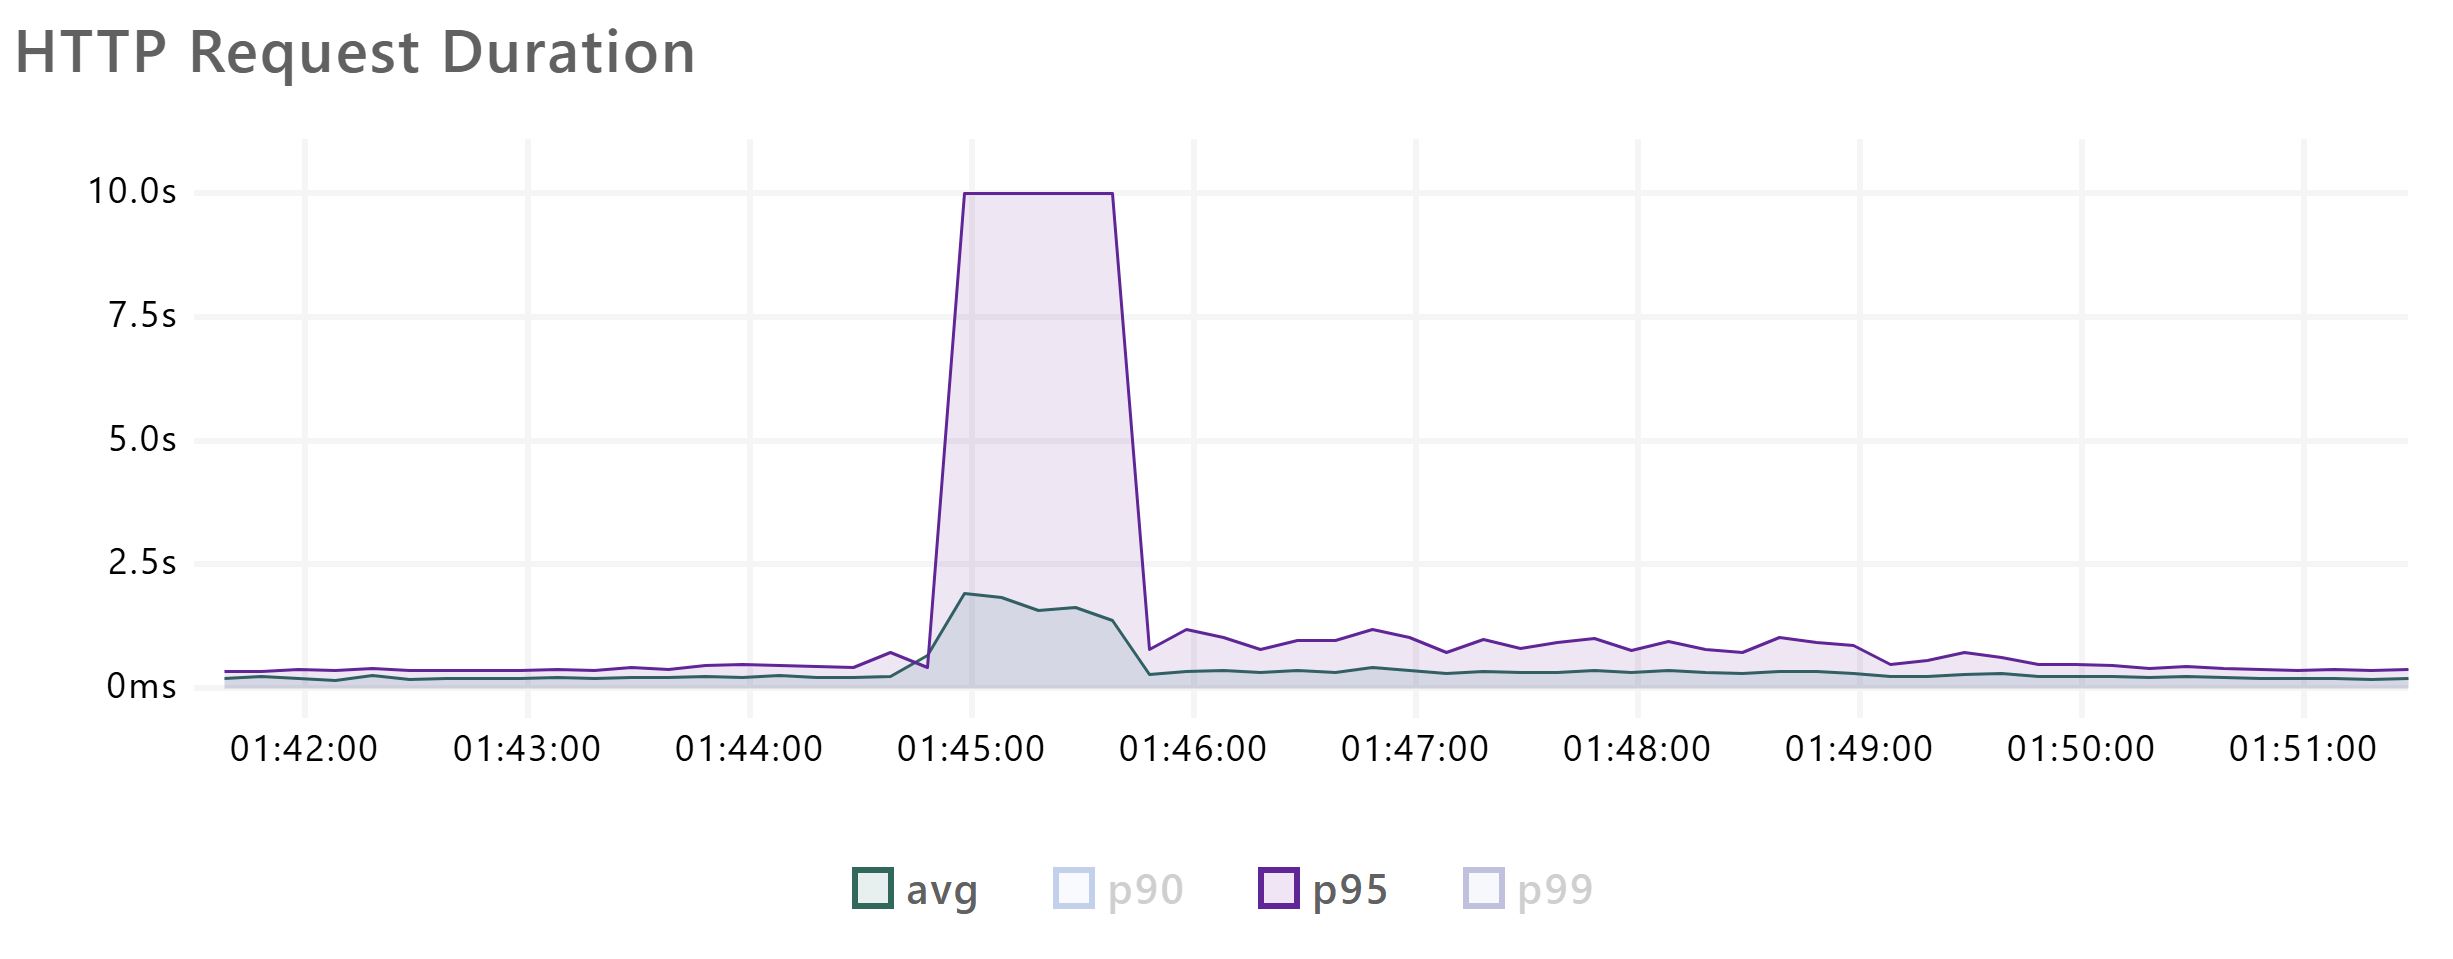
\includegraphics[width=1\textwidth]{assets/server-failing-test/req-duration.png}
    \caption{Duração das requisições ao longo do teste de falha de servidor}
    \label{fig:server-failing-req-duration}
\end{figure}

A Figura \ref{fig:server-failing-req-failed-rate} detalha a taxa de requisições falhadas por segundo ao longo da execução do teste. Analisando o gráfico é possível observar que a taxa de falhas manteve-se em torno de 0,2 requisição por segundo, representando menos de 1\% do total processado, com um pico de 0,34 requisição por segundo durante o período de falha. Após a identificação do servidor com falha, os valores retornaram aos níveis normais, indicando que a infraestrutura foi capaz de lidar com a falha sem impactar significativamente a operação da plataforma.

\begin{figure}[H]
    \centering
    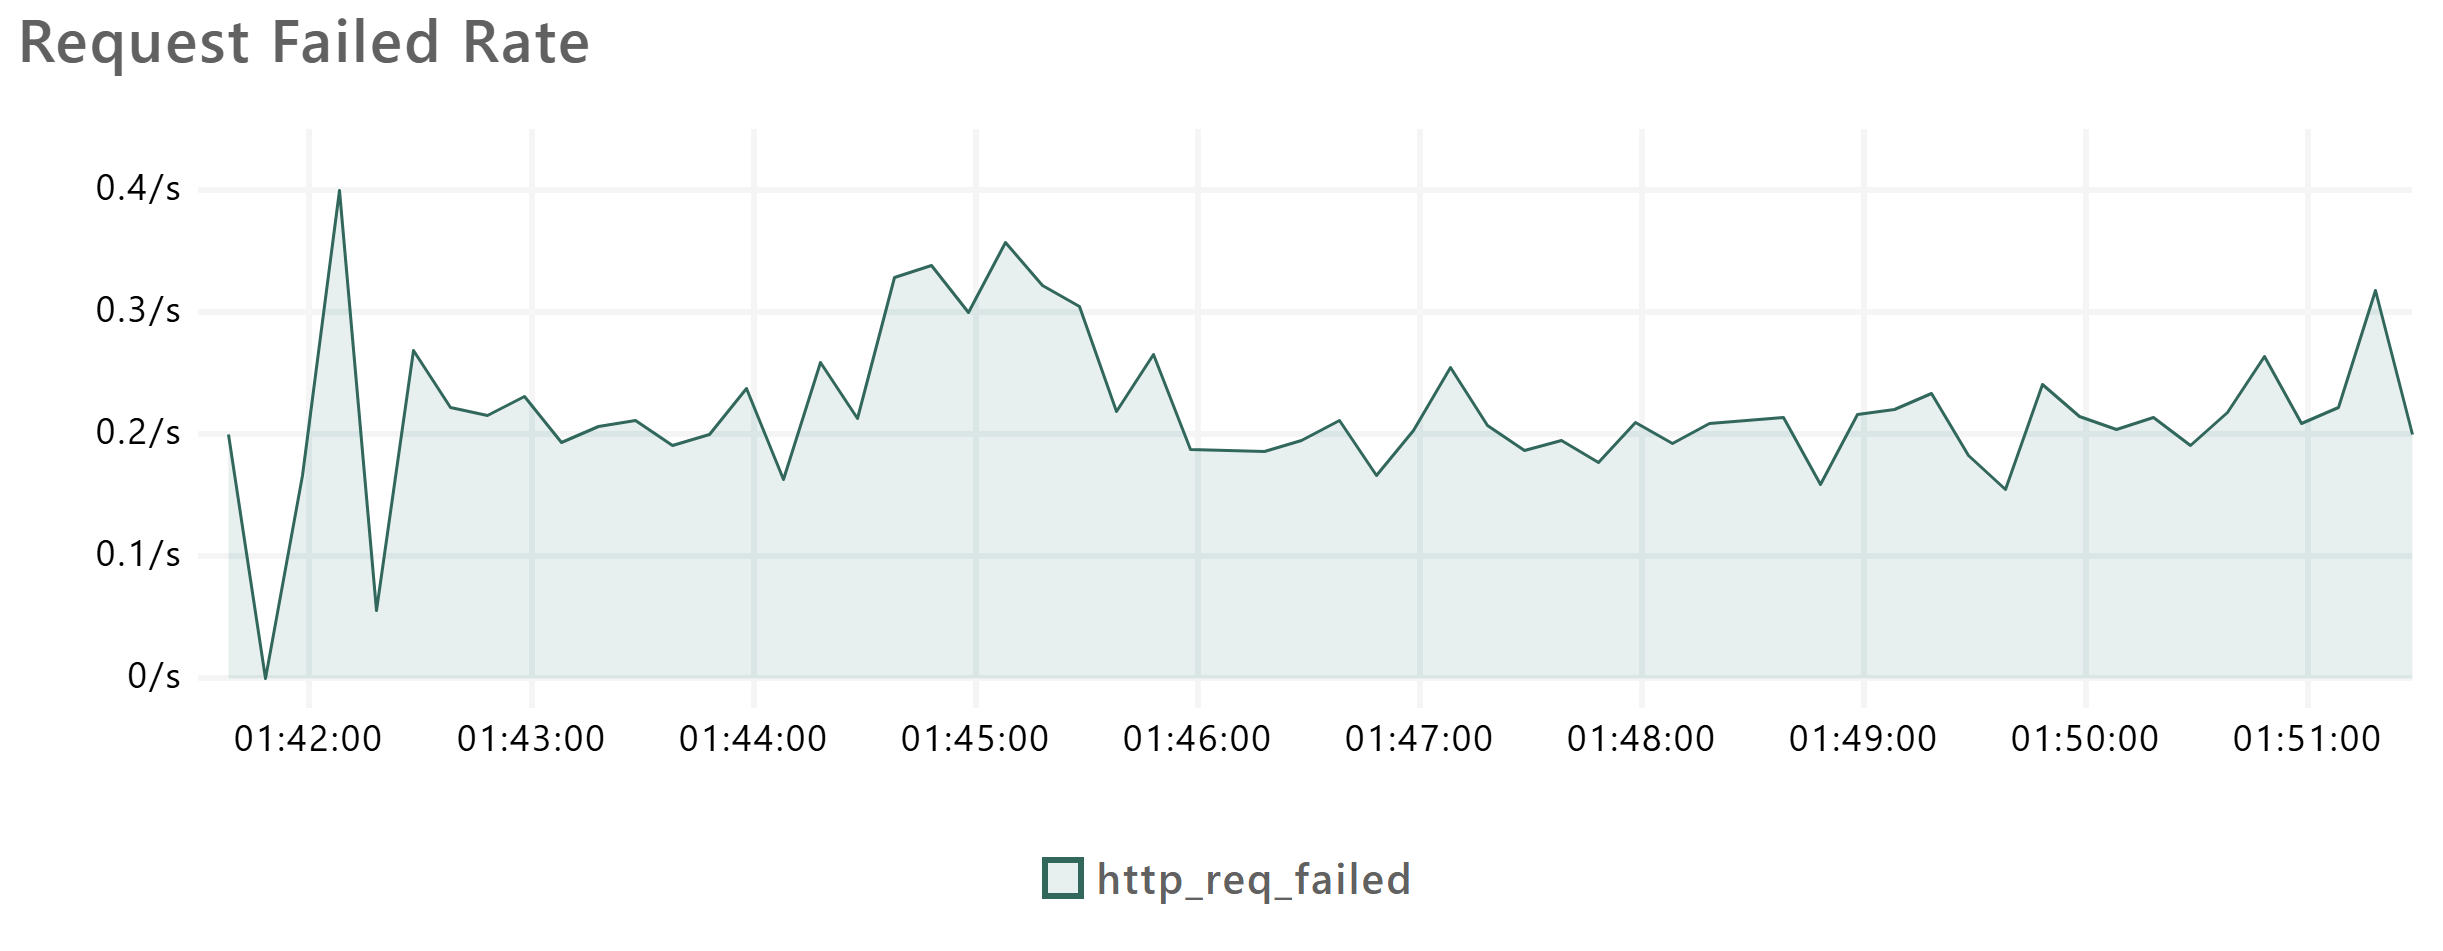
\includegraphics[width=1\textwidth]{assets/server-failing-test/req-failed-rate.png}
    \caption{Taxa de requisições falhadas ao longo do teste de falha de servidor}
    \label{fig:server-failing-req-failed-rate}
\end{figure}

A Figura \ref{fig:server-failing-healthy-hosts} detalha a quantidade de servidores disponíveis ao longo do tempo. Durante o teste, o número caiu de dois para um após o desligamento manual às 01:44. Um novo servidor foi provisionado automaticamente e tornou-se funcional às 01:47, restaurando a capacidade total da infraestrutura.

\begin{figure}[H]
    \centering
    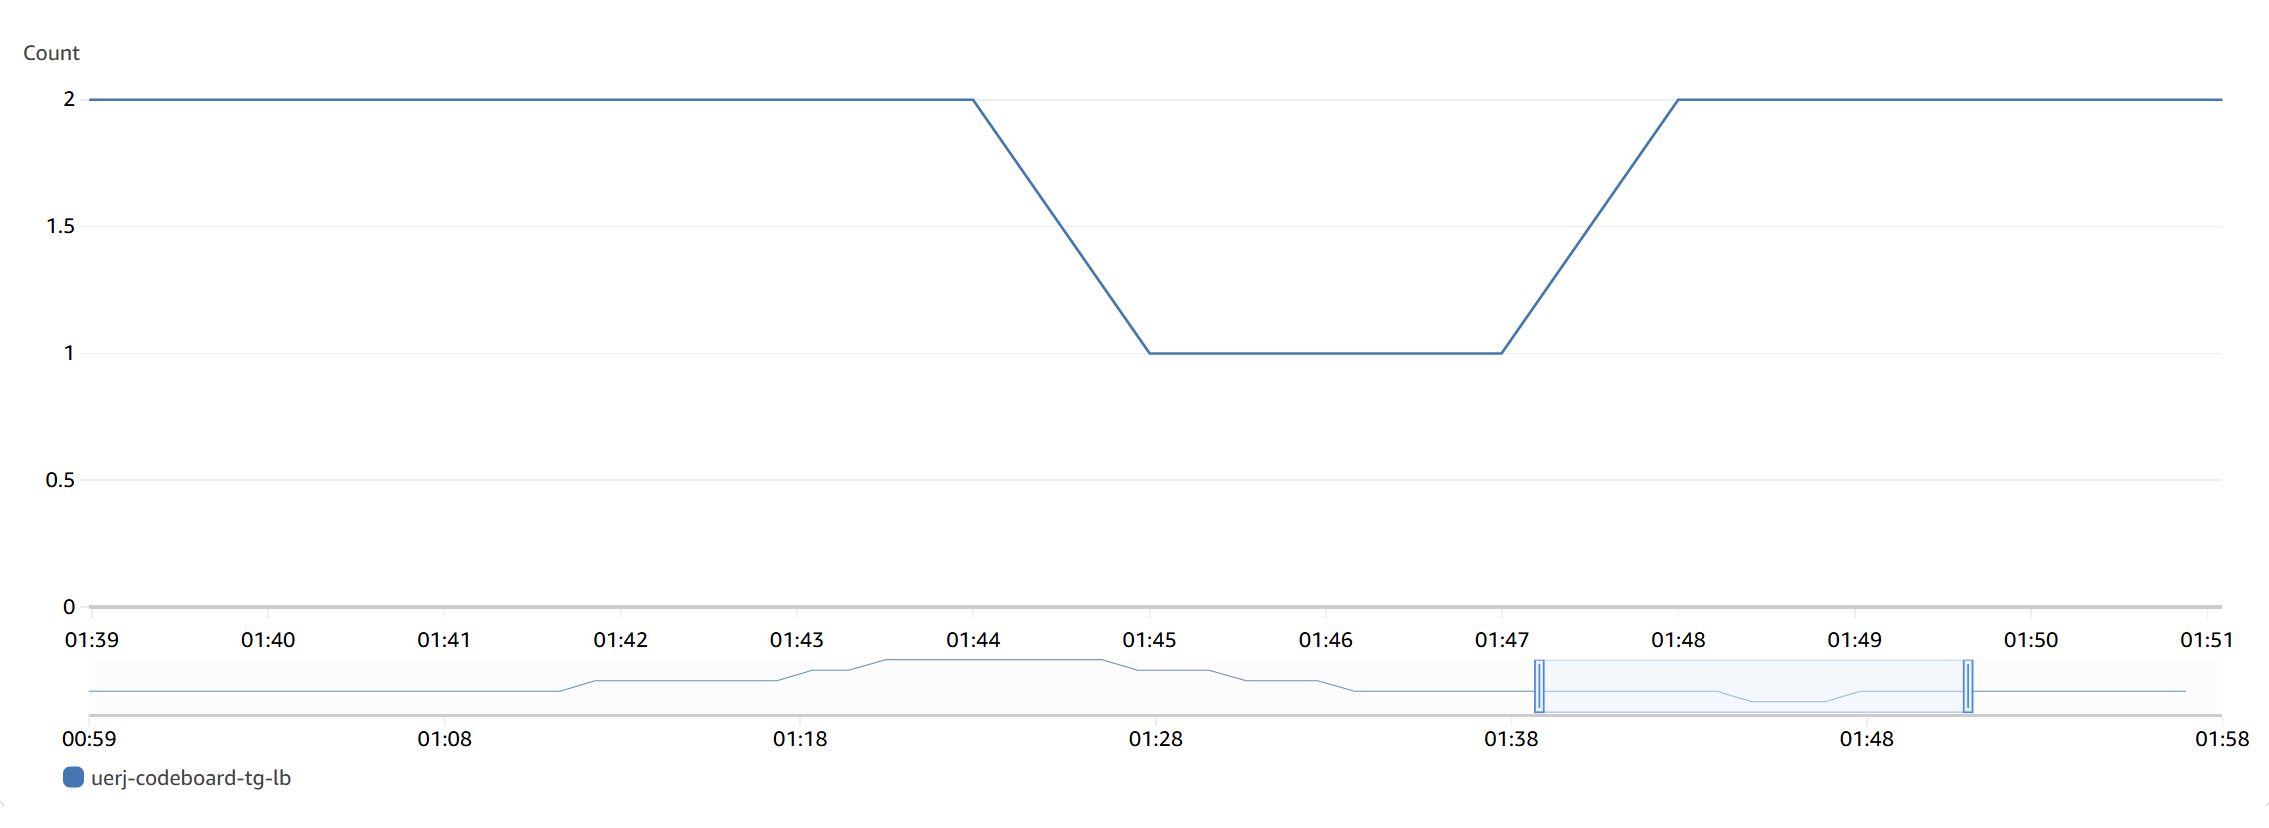
\includegraphics[width=1\textwidth]{assets/server-failing-test/healthy-hosts.png}
    \caption{Número de servidores disponíveis ao longo do teste de falha de servidor}
    \label{fig:server-failing-healthy-hosts}
\end{figure}

\subsection{Falhas da Aplicação}

Neste experimento, foi simulada uma falha na aplicação encerrando manualmente todos os dois processos de um servidor por meio de comandos no terminal, utilizando conexão SSH e o comando \texttt{kill -9 <PID>}. O objetivo foi avaliar a capacidade da infraestrutura de recuperar automaticamente os processos encerrados, mantendo a disponibilidade da plataforma.

A Figura \ref{fig:process-failing-vus-and-reqs} apresenta a evolução do número de usuários simultâneos e da taxa de requisições processadas por segundo ao longo do teste. Diferentemente do teste de falha de servidor, a taxa de requisições se manteve estável ao longo do experimento, indicando que a aplicação conseguiu reiniciar automaticamente o processo encerrado, garantindo a continuidade do serviço.

\begin{figure}[H]
    \centering
    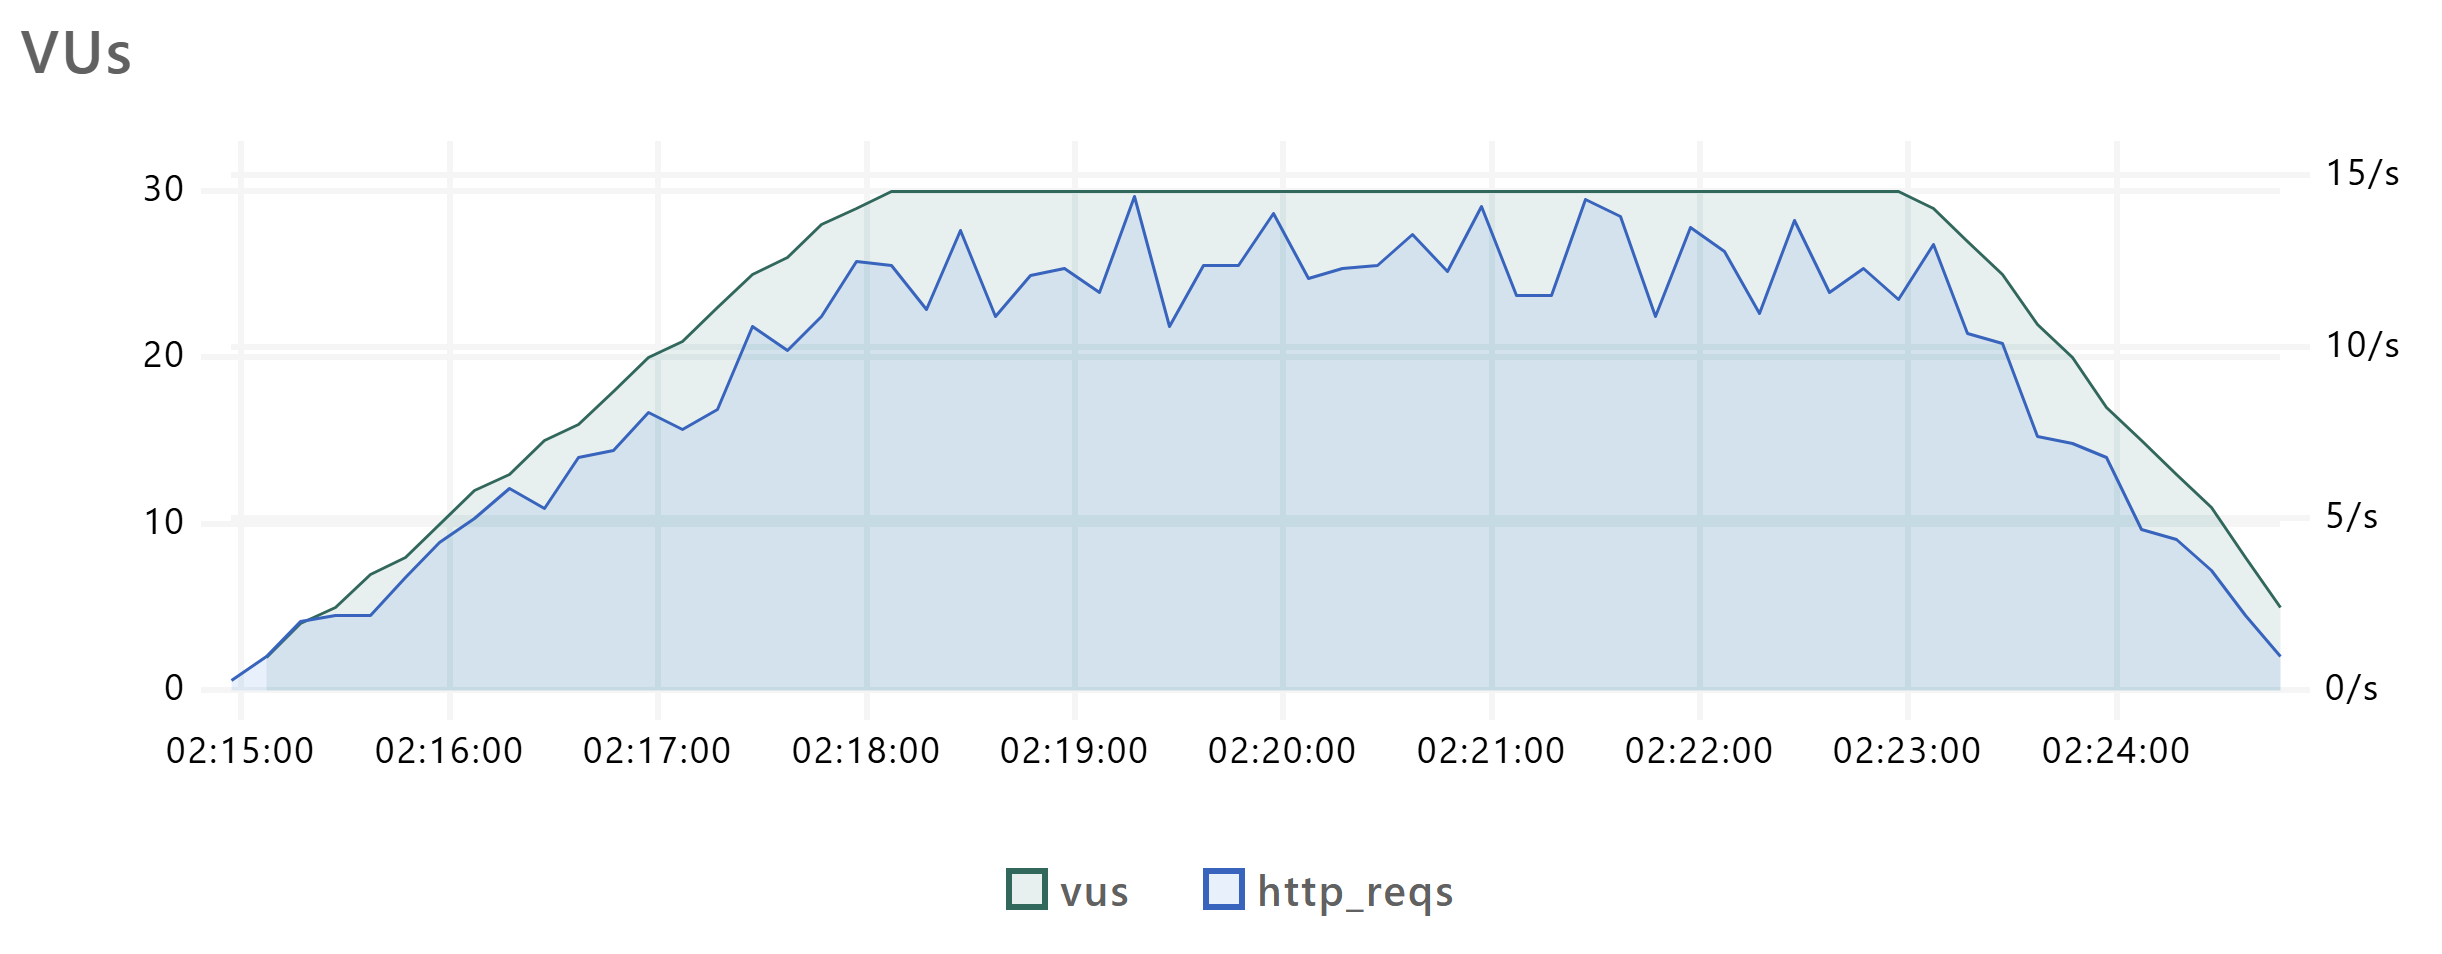
\includegraphics[width=1\textwidth]{assets/process-failing-test/vus-and-reqs.png}
    \caption{Número de usuários virtuais e taxa de requisições processadas por segundo ao longo do teste de falha de aplicação}
    \label{fig:process-failing-vus-and-reqs}
\end{figure}

A Figura \ref{fig:process-failing-req-duration} apresenta a evolução média e o percentil 95 das durações das requisições ao longo do teste. A duração média das requisições manteve-se próxima de 250 ms, exceto por um aumento temporário para 730 ms no momento da falha, registrada às 02:19:17. Esse impacto foi rapidamente mitigado, com os tempos de resposta retornando à normalidade em menos de 10 segundos após o incidente. O percentil 95, que reflete o tempo das 5\% requisições mais lentas, não apresentou alterações significativas durante o teste, indicando que a falha não afetou significativamente os tempos de resposta e, possivelmente, passou despercebida pelos usuários finais.

\begin{figure}[H]
    \centering
    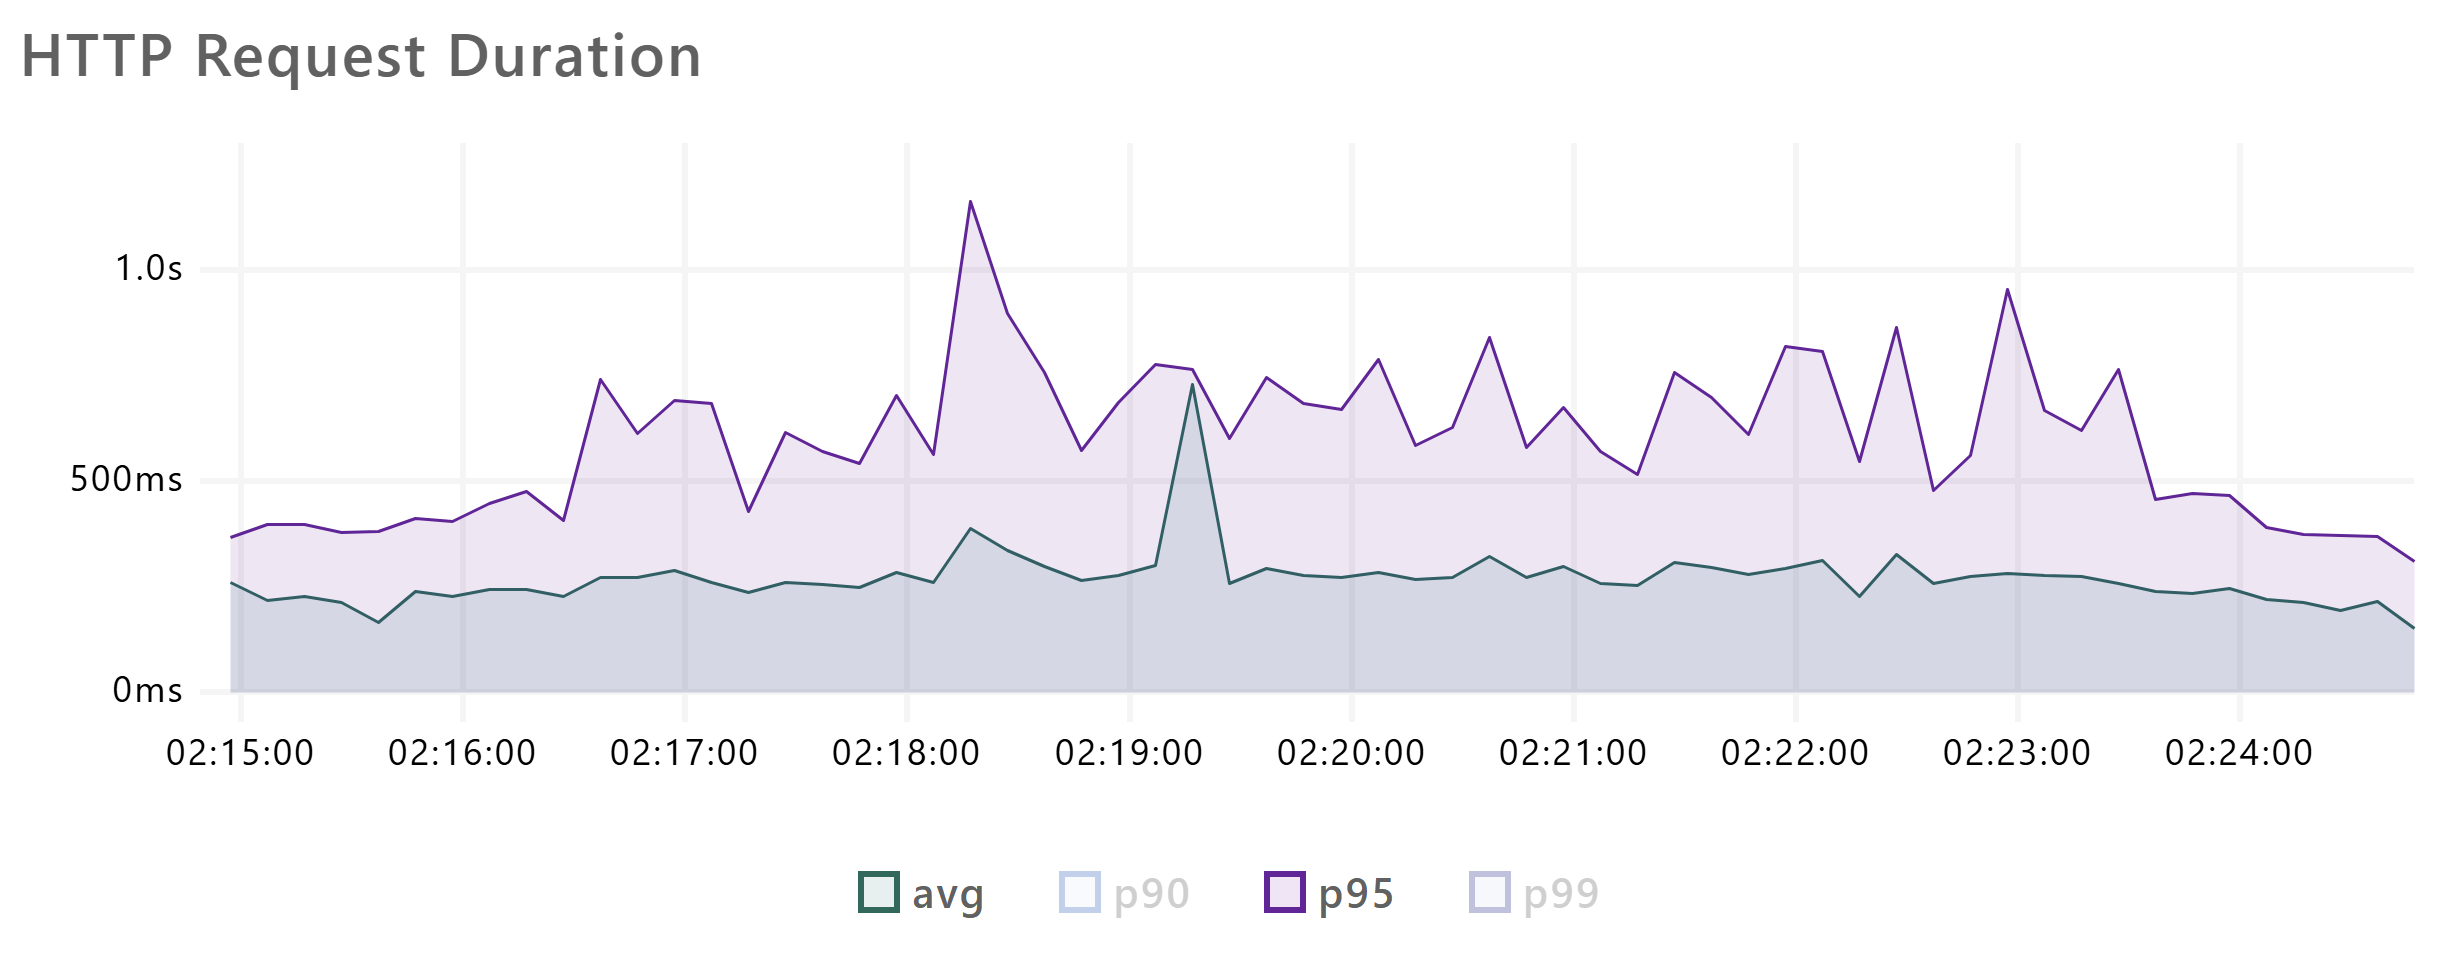
\includegraphics[width=1\textwidth]{assets/process-failing-test/req-duration.png}
    \caption{Duração das requisições ao longo do teste de falha de servidor}
    \label{fig:process-failing-req-duration}
\end{figure}

A Figura \ref{fig:process-failing-req-failed-rate} mostra a taxa de requisições falhadas por segundo ao longo do teste. Observa-se que a taxa de falhas se manteve estável em aproximadamente 0,2 falhas por segundo, sem aumentos significativos, mesmo durante o período da falha. Esse comportamento reforça a resiliência da aplicação, garantindo que o impacto do incidente foi minimizado.

\begin{figure}[H]
    \centering
    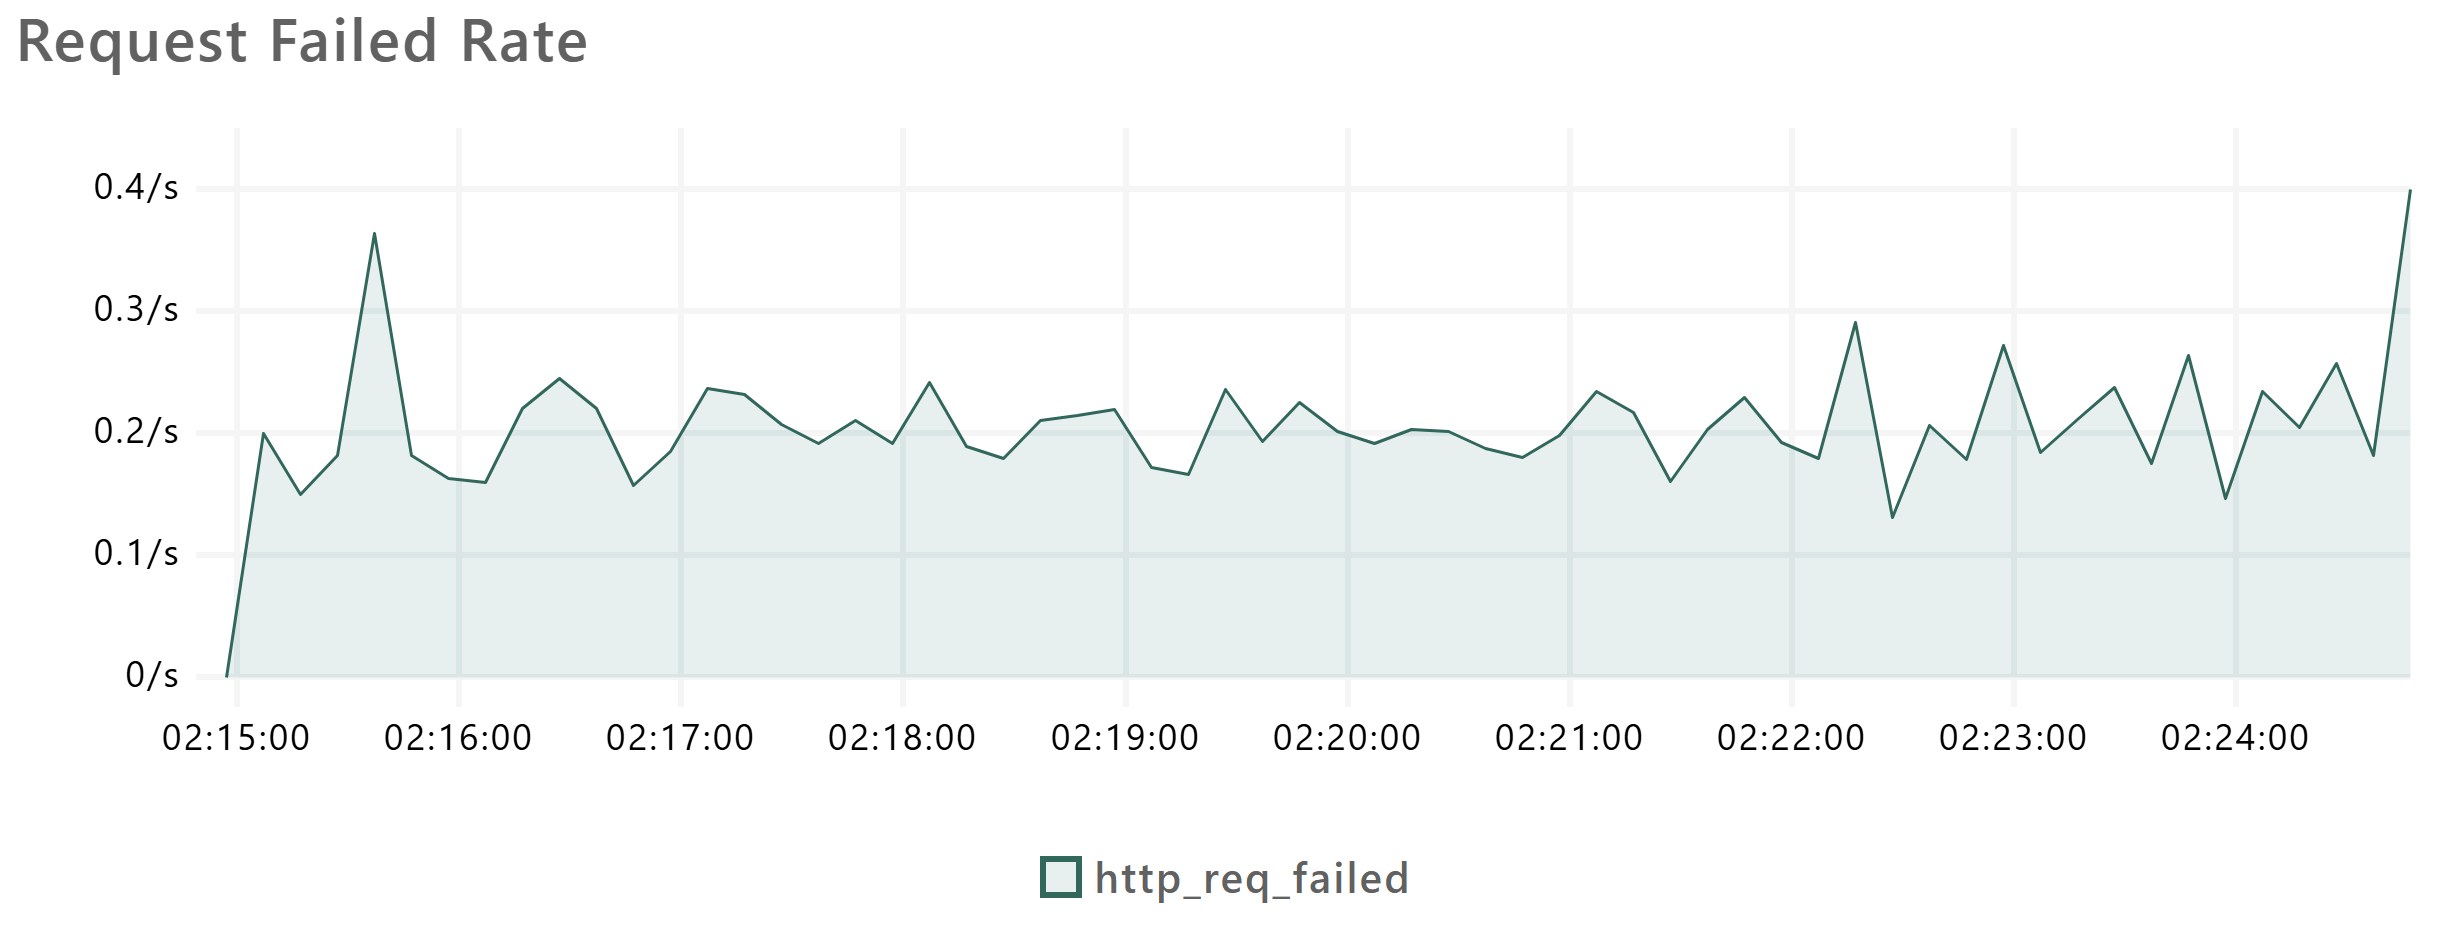
\includegraphics[width=1\textwidth]{assets/process-failing-test/req-failed-rate.png}
    \caption{Taxa de requisições falhadas ao longo do teste de falha de servidor}
    \label{fig:process-failing-req-failed-rate}
\end{figure}

A Figura \ref{fig:process-failing-healthy-hosts} detalha a quantidade de servidores disponíveis durante o teste. Nota-se que a infraestrutura permaneceu estável, mantendo dois servidores disponíveis ao longo de todo o período, evidenciando que a falha na aplicação não comprometeu a disponibilidade geral. Os processos encerrados (PIDs 1616 e 1627) foram rapidamente substituídos pelos novos processos (PIDs 3127 e 3146), comprovando a eficácia do mecanismo de recuperação automática da aplicação em garantir a continuidade do serviço.

\begin{figure}[H]
    \centering
    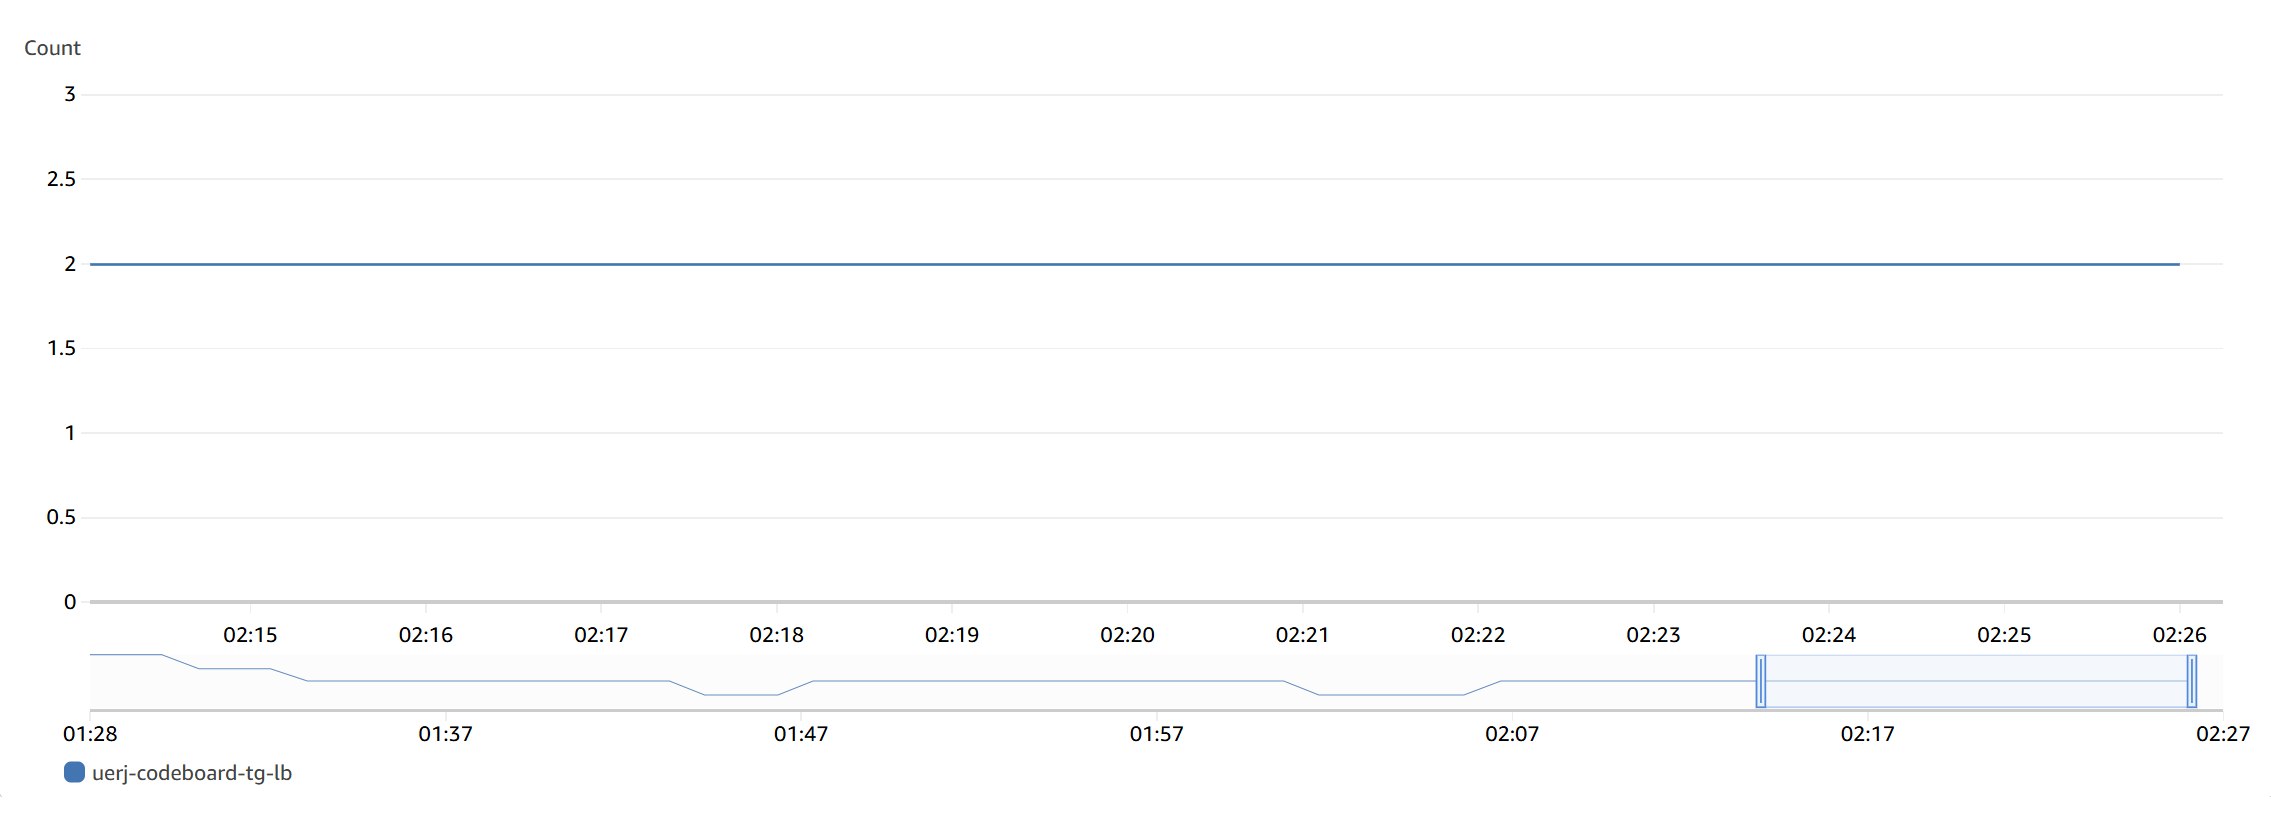
\includegraphics[width=1\textwidth]{assets/process-failing-test/healthy-hosts.png}
    \caption{Número de servidores disponíveis ao longo do teste de falha de servidor}
    \label{fig:process-failing-healthy-hosts}
\end{figure}


\section{Testes de Segurança}
% OK

A segurança é um aspecto crítico para qualquer aplicação web. Nesta seção, são apresentados os testes realizados para identificar vulnerabilidades e assegurar a proteção dos dados dos usuários na plataforma Codeboard UERJ.

\subsection{Testes de Firewall}

Para avaliar a configuração e eficácia das regras de firewall, foi utilizado o \emph{Nmap} \cite{nmap}, uma ferramenta de análise de segurança. O comando \texttt{nmap -p- -sV -O -Pn -T4 <DOMAIN>} permitiu realizar um escaneamento de portas, identificando aquelas que estavam abertas e verificando se apenas as portas essenciais para o funcionamento da aplicação estavam acessíveis. Os resultados obtidos estão apresentados na Figura \ref{fig:nmap-scan}.

\begin{figure}[H]
    \centering
    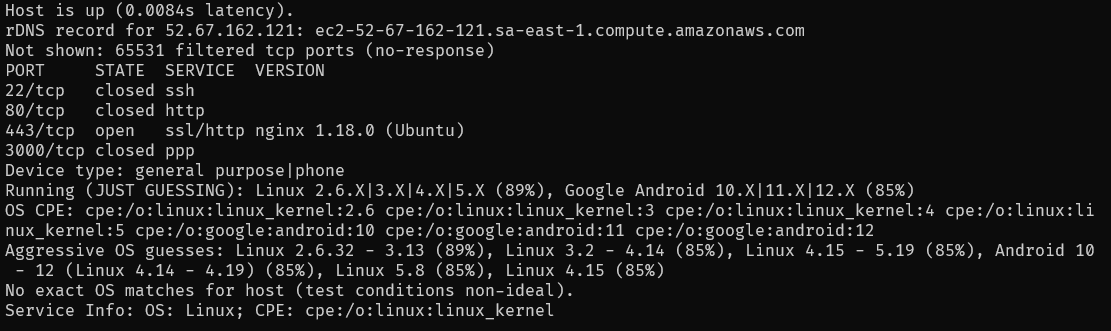
\includegraphics[width=1\textwidth]{assets/security-test/nmap-scan.png}
    \caption{Resultado do escaneamento de portas com o Nmap}
    \label{fig:nmap-scan}
\end{figure}

Como ilustrado na Figura \ref{fig:nmap-scan}, o escaneamento revelou que somente a porta 443, utilizada para comunicações seguras via HTTPS, estava aberta. Todas as demais portas permaneceram fechadas. Este resultado demonstra que a infraestrutura está adequadamente protegida contra acessos não autorizados e possíveis ataques de rede, garantindo a segurança dos dados dos usuários.

\subsection{Criptografia em Trânsito}

Para assegurar a segurança das comunicações entre clientes e servidores, foi utilizado o serviço \emph{SSL Labs} \cite{ssl-labs}, que realiza uma análise detalhada da configuração de segurança do servidor e da qualidade da criptografia em trânsito. Este teste foi realizado para confirmar a integridade e a confidencialidade dos dados transmitidos pela plataforma. A Figura \ref{fig:ssl-labs} apresenta o resultado da análise feita pelo SSL Labs.

\begin{figure}[H]
    \centering
    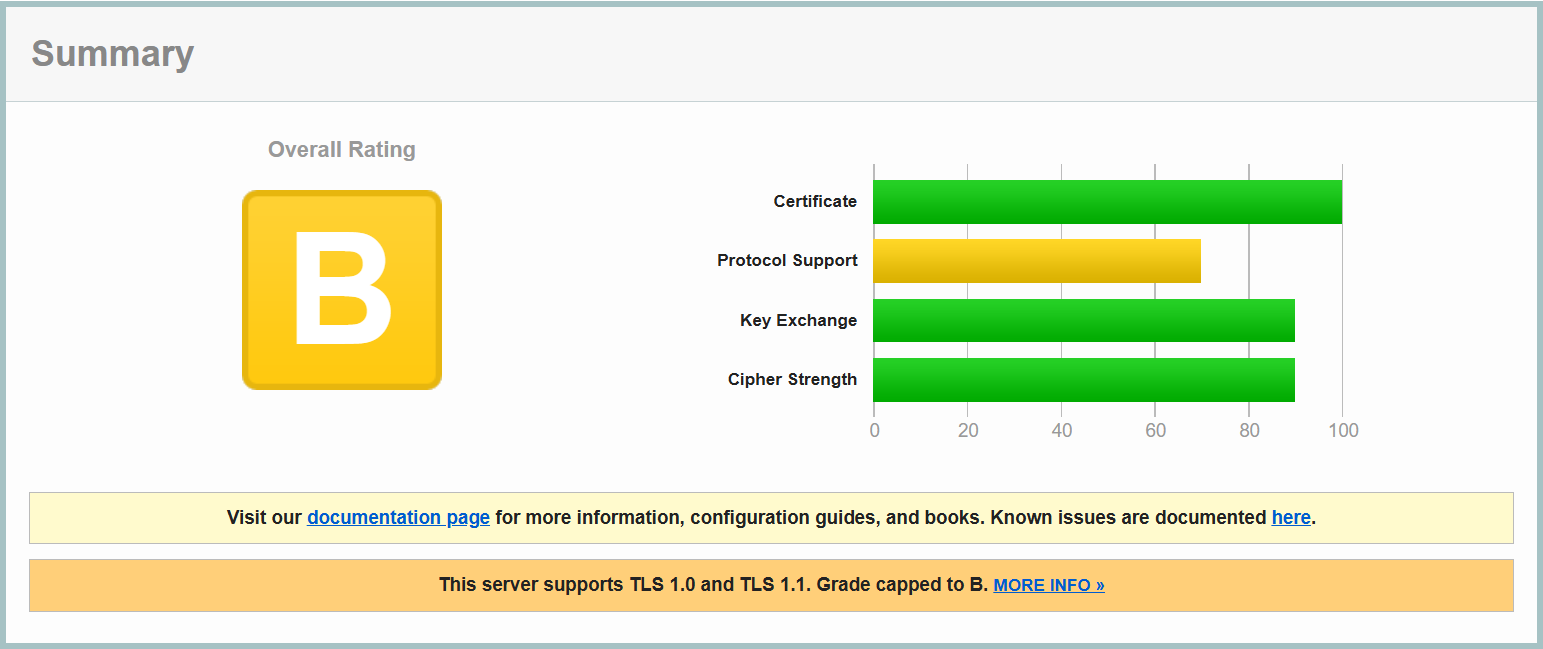
\includegraphics[width=1\textwidth]{assets/security-test/ssl-labs.png}
    \caption{Resultado do teste de criptografia em trânsito com o SSL Labs}
    \label{fig:ssl-labs}
\end{figure}

Conforme mostrado na Figura \ref{fig:ssl-labs}, a plataforma Codeboard UERJ obteve a classificação "B" no teste. Isso indica que, embora a configuração de segurança seja satisfatória, há margem para melhorias. Recomendações feitas pelo site incluíram a desativação de protocolos obsoletos, como TLS 1.0 e 1.1, e a implementação de políticas de segurança mais rigorosas para alcançar um nível mais elevado de proteção.


\section{Monitoramento}

O monitoramento contínuo da infraestrutura é fundamental para a detecção prévia de problemas e para a manutenção da disponibilidade e desempenho da plataforma de forma proativa. Nesta seção, apresentamos os testes de monitoramento realizados na plataforma Codeboard UERJ.

\subsection{Monitoramento de Recursos}

O uso eficiente dos recursos é essencial para a manutenção de uma infraestrutura escalável e econômica. O serviço Amazon CloudWatch foi utilizado para monitorar o uso de CPU, memória e armazenamento das instâncias EC2, permitindo identificar gargalos de desempenho e otimizar a alocação de recursos. A Figura \ref{fig:elasticity-cpu-usage} exemplifica esse monitoramento, apresentando o gráfico de uso de CPU das instâncias EC2 durante os testes de elasticidade.

\begin{figure}[H] 
    \centering 
    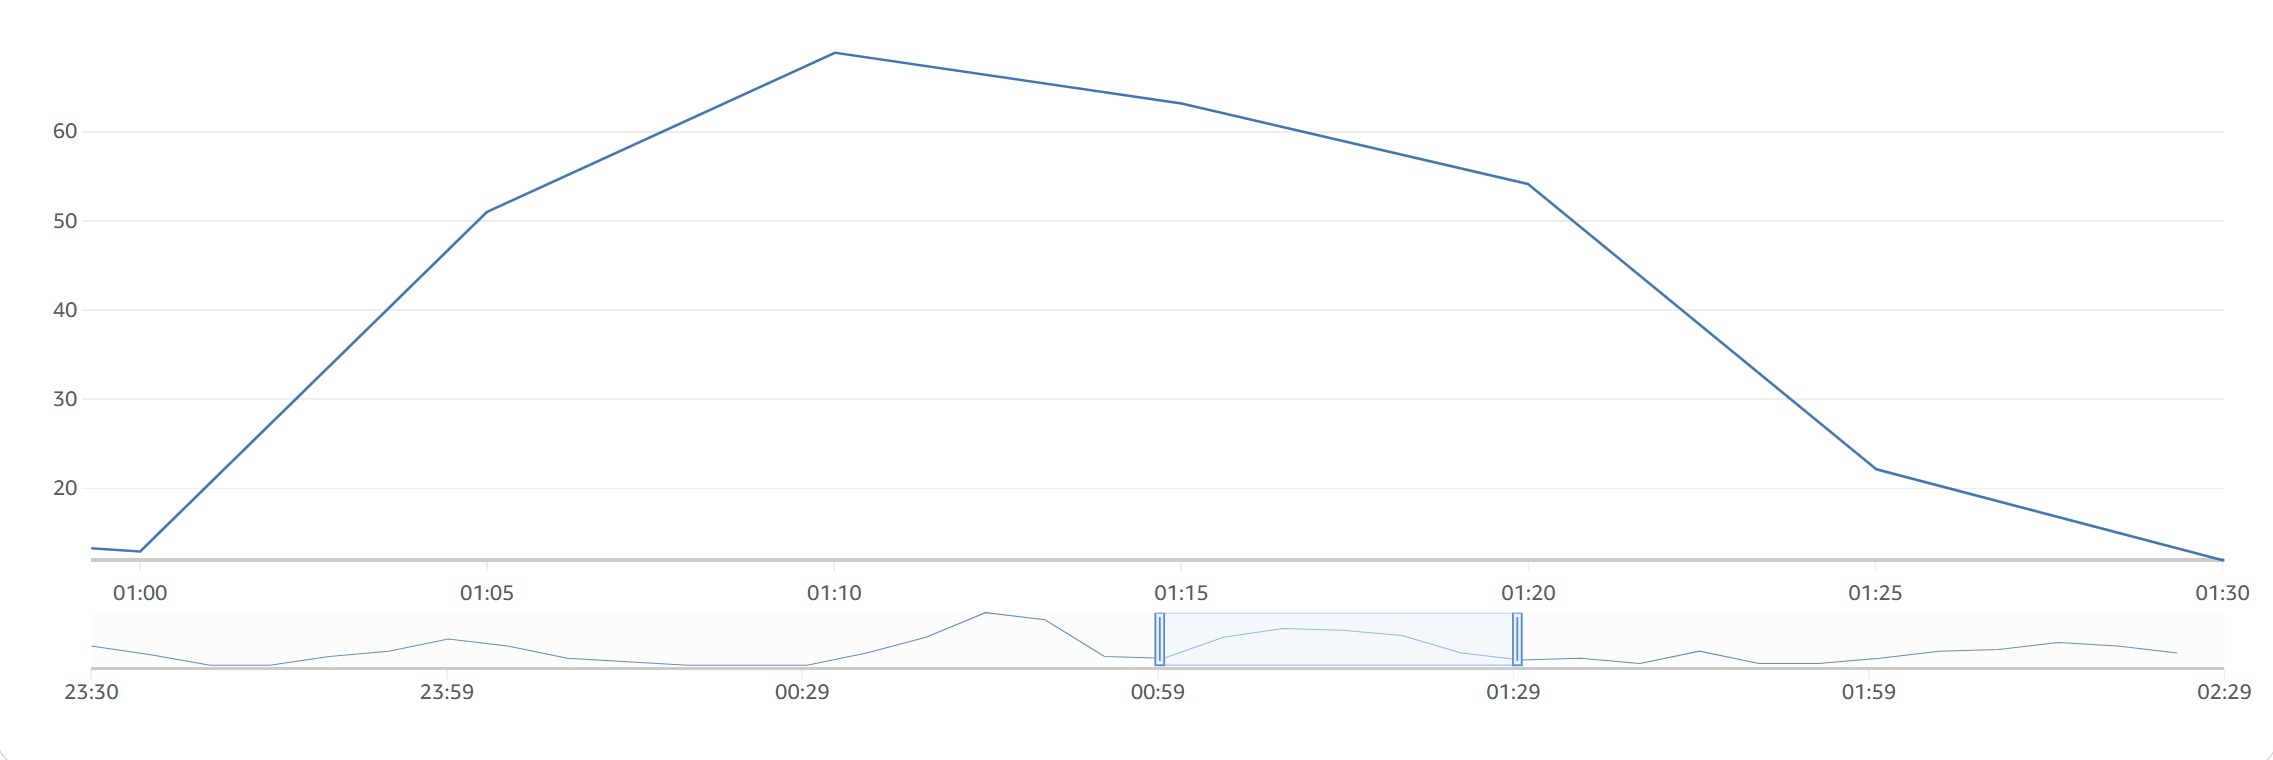
\includegraphics[width=1\textwidth]{assets/elasticity-test/cpu-usage.png}
    \caption{Gráfico de uso de CPU das instâncias EC2 durante o teste de elasticidade}
    \label{fig:elasticity-cpu-usage} 
\end{figure}

Observando a Figura \ref{fig:elasticity-cpu-usage}, foi possível identificar o aumento do uso de CPU das instâncias durante os testes de elasticidade, com picos acima de 60\% de utilização. Essas informações permitem uma análise detalhada do desempenho da infraestrutura e a tomada de decisões informadas para otimização dos recursos.

\subsection{Monitoramento de Logs}

O monitoramento de logs é uma prática indispensável para identificar padrões suspeitos, diagnosticar falhas e rastrear eventos críticos no sistema. Um exemplo ilustrativo de logs gerados pelo Amazon CloudWatch é apresentado na Figura \ref{fig:cloudwatch-logs}.

\begin{figure}[H]
    \centering
    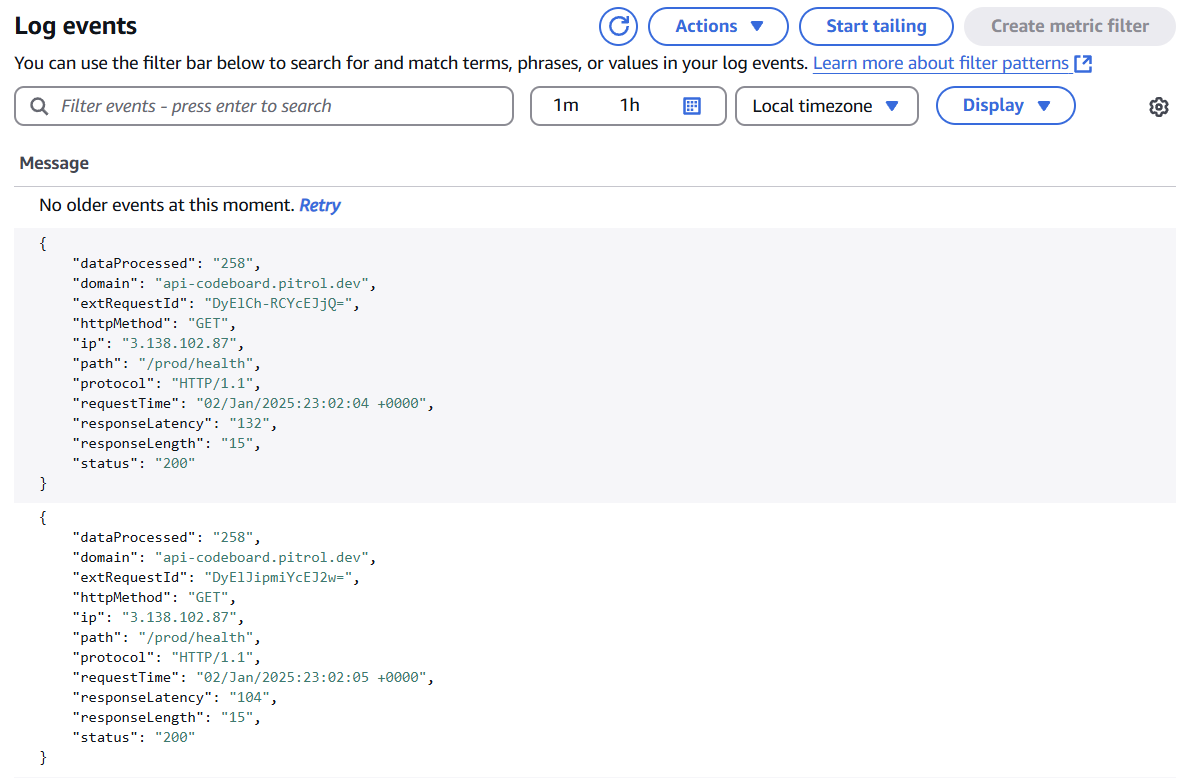
\includegraphics[width=1\textwidth]{assets/monitoring-test/cloudwatch-logs.png}
    \caption{Exemplo de logs enviados ao Amazon CloudWatch}
    \label{fig:cloudwatch-logs}
\end{figure}

A análise dos logs pode fornecer informações importantes sobre o comportamento do sistema, como requisições de API, erros de aplicação e atividades de usuários. Esses dados normalmente são utilizados para identificar problemas, otimizar o desempenho ou auditar ações realizadas na plataforma.

\subsection{Alertas de Incidentes}

Para assegurar respostas rápidas a eventos críticos, foram configurados alertas automatizados utilizando o Amazon CloudWatch integrado ao Amazon SNS. Esses alertas são acionados sempre que métricas predefinidas, como uso elevado de CPU ou taxas de erro acima do aceitável, ultrapassam os limites estabelecidos.

A Figura \ref{fig:cloudwatch-alarm-config} mostra a configuração de um alarme no Amazon CloudWatch para monitorar a quantidade de requisições processadas em um período de um minuto. Quando o limite de 50 requisições é ultrapassado, o alarme é acionado e uma notificação é enviada automaticamente para o tópico do Amazon SNS.

\begin{figure}[H]
    \centering
    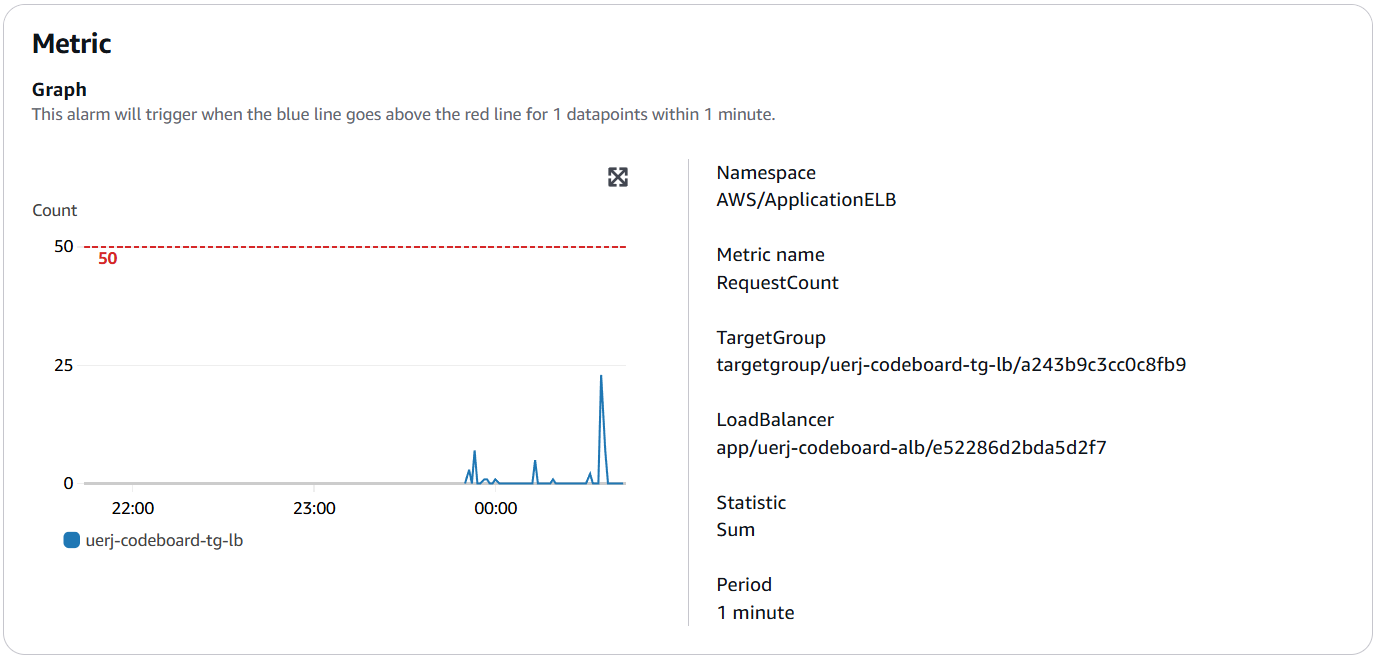
\includegraphics[width=1\textwidth]{assets/monitoring-test/cloudwatch-alarm-config.png}
    \caption{Alarme configurado no Amazon CloudWatch}
    \label{fig:cloudwatch-alarm-config}
\end{figure}

Já a Figura \ref{fig:cloudwatch-alarm-email} apresenta um exemplo de e-mail de alerta enviado pelo Amazon SNS em resposta a um evento de alta quantidade de requisições. Esses alertas permitem que a equipe técnica seja notificada em tempo real sobre qualquer anomalia operacional, reduzindo significativamente o tempo de resposta para a resolução de problemas.

\begin{figure}[H]
    \centering
    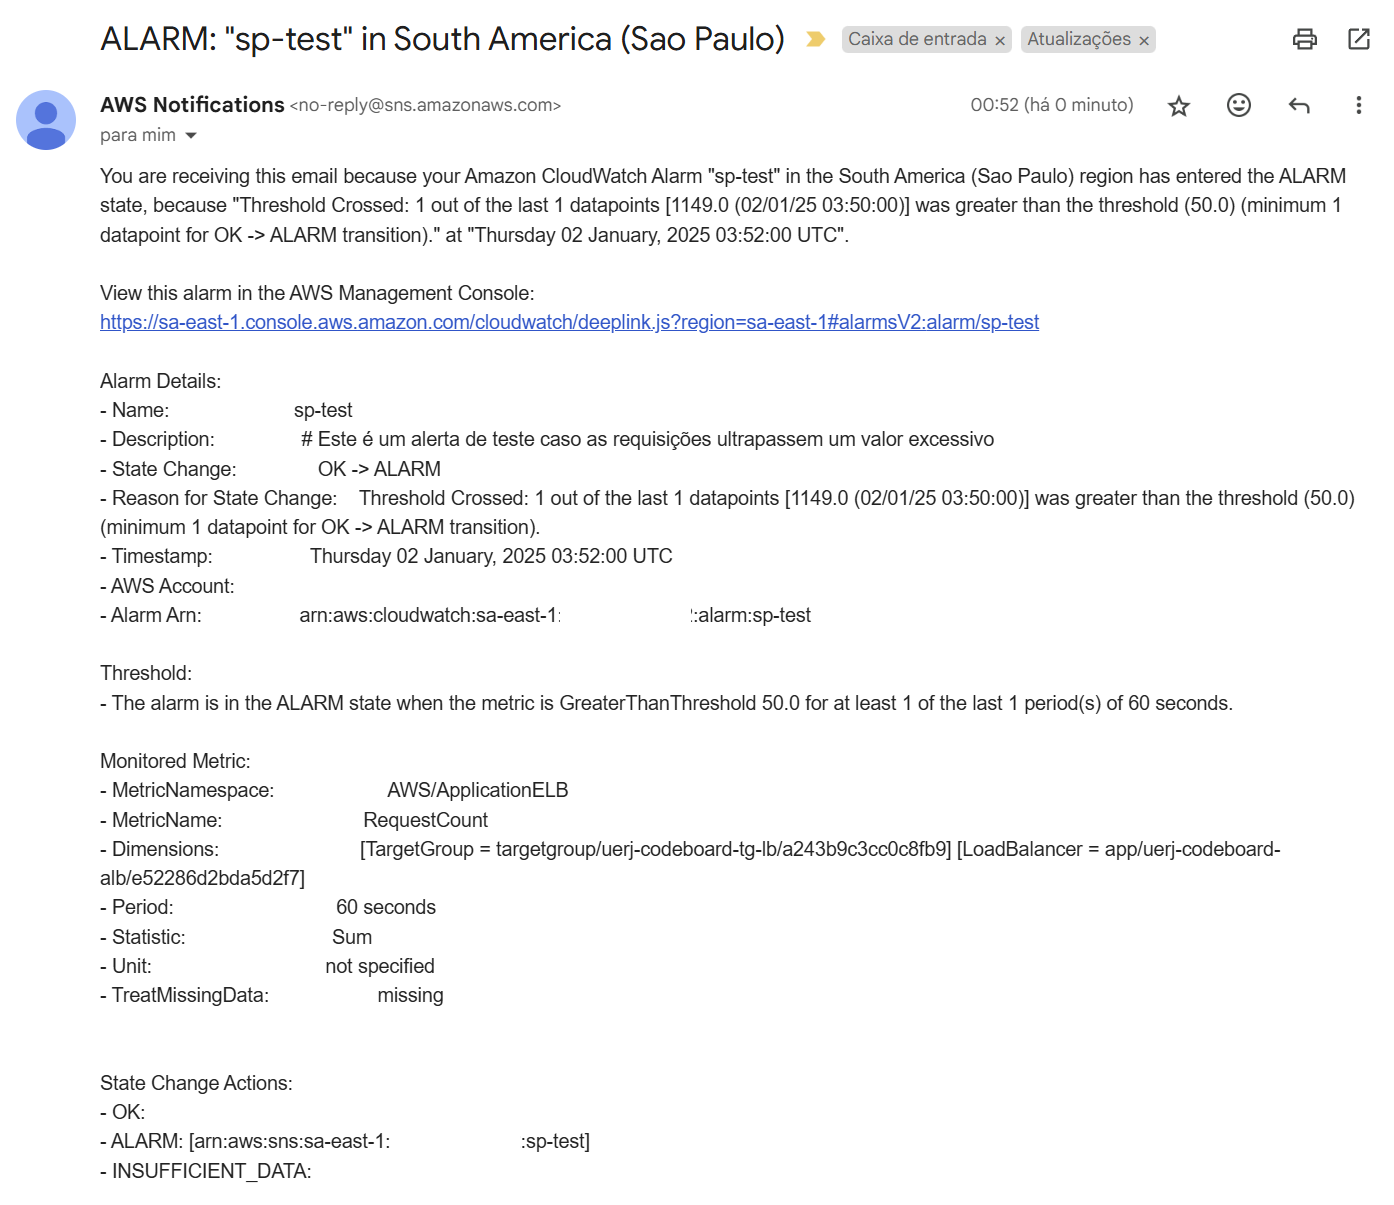
\includegraphics[width=1\textwidth]{assets/monitoring-test/cloudwatch-alarm-email.png}
    \caption{Exemplo de e-mail de alerta do Amazon SNS}
    \label{fig:cloudwatch-alarm-email}
\end{figure}

Por exemplo, durante um pico inesperado de tráfego, os alertas viabilizam a ativação imediata de instâncias adicionais, assegurando a continuidade dos serviços. Essa abordagem proativa minimiza impactos nos usuários e garante a estabilidade da plataforma.
